\documentclass[a4paper,oneside,titlepage,10pt]{article}


\usepackage{xltxtra}
\usepackage{xgreek}
\setmainfont[Mapping=tex-text]{Calibri.ttf} %Courier New for programing
\usepackage{amsfonts}
\usepackage{listings}



%\setmainfont[Mapping=tex-text]{Helvetica}
\setmainfont[Mapping=tex-text]{Calibri.ttf}
\setmainfont[
 BoldFont={CALIBRIB.TTF}, 
 ItalicFont={CALIBRII.TTF},
 BoldItalicFont={CALIBRIZ.TTF}
 ]{Calibri.ttf}
 
 \usepackage{amsmath}

\usepackage{alltt}



\usepackage[margin=1in]{geometry}

% \usepackage[hidelinks]{hyperref}

%\usepackage[]{hyperref}

 \usepackage[colorlinks = true,
             linkcolor = black,
             urlcolor  = blue,
             citecolor = blue,
            anchorcolor = blue]{hyperref}

\usepackage{enumitem}


%\usepackage[LGR]{fontenc}

%\renewcommand{\familydefault}{\sfdefault}



\usepackage{graphicx,wrapfig}
\graphicspath{ {images/} }

\usepackage[usenames, dvipsnames]{color}
\definecolor{mygray}{gray}{0.6}

\usepackage[table,xcdraw]{xcolor}

\definecolor{calpolypomonagreen}{rgb}{0.07, 0.53, 0.03}


\usepackage{listings}

\lstdefinelanguage{diff}{
  morecomment=[f][\color{blue}]{@@},     % group identifier
  morecomment=[f][\color{red}]-,         % deleted lines 
  morecomment=[f][\color{calpolypomonagreen}]+,       % added lines
  morecomment=[f][\color{magenta}]{---}, % Diff header lines (must appear after +,-)
  morecomment=[f][\color{magenta}]{+++},
}

\lstdefinelanguage{diffrrr}{
  sensitive=true,
  % diff command line
  morecomment=[f][\color{gray}][0]{diff},
  % commit identifiers for git diff
  morecomment=[f][\color{gray}][0]{index},
  % hunk location/line numbers for unified format
  morecomment=[f][\color{blue}][0]{@@},
  % hunk location/line numbers for context format
  morecomment=[f][\color{magenta}][0]{***},
  % changed line for context format
  morecomment=[f][\color{violet}][0]{!},
  % deleted lines for unified format
  morecomment=[f][\color{red!60!black}][0]-,
  % added lines for unified format
  morecomment=[f][\color{green!60!black}][0]+,
  % file name and time stamp old file
  morecomment=[f][\color{magenta}][0]{---},
  % file name and time stamp new file
  morecomment=[f][\color{magenta}][0]{+++},
  % Binary files ... differ
  morecomment=[f][\color{gray}][0]{Binary},
  % Only in ...: file.txt
  morecomment=[f][\color{gray}][0]{Only},
  % old mode ...
  morecomment=[f][\color{gray}][0]{old},
  % new mode ...
  morecomment=[f][\color{gray}][0]{new},
  % rename from/to ...
  morecomment=[f][\color{gray}][0]{rename},
  % similarity index ...%
  morecomment=[f][\color{gray}][0]{similarity},
  % deleted file mode ...%
  morecomment=[f][\color{gray}][0]{deleted},
  % hunk separator for context format
  morecomment=[f][\color{magenta}][0]{***************},
  % deleted lines for normal format
  morecomment=[f][\color{red!60!black}][0]<,
  % added lines for normal format
  morecomment=[f][\color{green!60!black}][0]>,
  % line number specifier for normal format
  morecomment=[f][\color{blue}][0]{0},
  % line number specifier for normal format
  morecomment=[f][\color{blue}][0]{1},
  % line number specifier for normal format
  morecomment=[f][\color{blue}][0]{2},
  % line number specifier for normal format
  morecomment=[f][\color{blue}][0]{3},
  % line number specifier for normal format
  morecomment=[f][\color{blue}][0]{4},
  % line number specifier for normal format
  morecomment=[f][\color{blue}][0]{5},
  % line number specifier for normal format
  morecomment=[f][\color{blue}][0]{6},
  % line number specifier for normal format
  morecomment=[f][\color{blue}][0]{7},
  % line number specifier for normal format
  morecomment=[f][\color{blue}][0]{8},
  % line number specifier for normal format
  morecomment=[f][\color{blue}][0]{9},
}[comments]

\definecolor{verbgray}{gray}{0.93}




\lstdefinestyle{myCustomMatlabStyle}{
  language=diff,
  backgroundcolor=\color{verbgray},
  stepnumber=1,
  numbersep=10pt,
  tabsize=4,
  showspaces=false,
  keepspaces=true,
  showstringspaces=false,
  frame=single,
  framerule=0pt,
  columns=fullflexible,
  basicstyle=\ttfamily\footnotesize
}

\lstdefinestyle{myCustomCStyle}{
  language=C,
  backgroundcolor=\color{verbgray},
  stepnumber=1,
  numbersep=10pt,
  tabsize=4,
  showspaces=false,
  showstringspaces=false,
  frame=single,
  framerule=0pt,
  columns=fullflexible,
  basicstyle=\ttfamily\footnotesize
}

\lstdefinestyle{CStyle}{
    backgroundcolor=\color{verbgray},   
    commentstyle=\color{green},
    keywordstyle=\color{magenta},
    numberstyle=\tiny\color{gray}\ttfamily,
    numbers=left,
    stringstyle=\color{purple},
    basicstyle=\ttfamily\small,
    breakatwhitespace=false,         
    breaklines=true,                 
    captionpos=b,                    
    keepspaces=true,                 
    showspaces=false,                
    showstringspaces=false,
    showtabs=false,                  
    tabsize=4,
    columns=fullflexible,
                keywordstyle=\color{blue}\ttfamily,
                stringstyle=\color{red}\ttfamily,
                commentstyle=\color{calpolypomonagreen}\ttfamily,
                morecomment=[l][\color{magenta}]{\#}
    language=C
}

\lstdefinestyle{bash}{
    backgroundcolor=\color{black},   
    commentstyle=\color{white},
    keywordstyle=\color{white},
    stringstyle=\color{white},
    basicstyle=\ttfamily\color{white}\small,
    breakatwhitespace=false,         
    breaklines=true,                 
    %captionpos=b,                    
    keepspaces=true,                 
    showspaces=false,                
    showstringspaces=false,
    showtabs=false,                  
    tabsize=4,
    linewidth=15cm,
    language=C
    %columns=fullflexible,
}

\usepackage{afterpage}
\usepackage{pagecolor}
\usepackage{titlesec}
\titlelabel{\thetitle.\quad}

\usepackage{hyperref}

\begin{document}

\color{white}
\begin{center}
    \thispagestyle{empty}
    %\vspace{-0.5cm}
    
\includegraphics[scale=0.9]{logo-neg.jpg}
    \pagecolor{black}\afterpage{\restorepagecolor}
    
    \vspace{0.1cm}
    
    \textsc{\large Πολυτεχνική Σχολή \\ Τμήμα Μηχανικών Ηλεκτρονικών Υπολογιστών \& Πληροφορικής}
    
    \vspace{0.75cm}
    
    {\huge \noindent\textbf{Λογισμικό και Προγραμματισμός\\Συστημάτων Υψηλής Επίδοσης}
    \vspace{0.1cm}
\\ {\large \textbf{Εργασία Χειμερινού Εξαμήνου 2018-2019}}}

\vspace{1cm}
    
    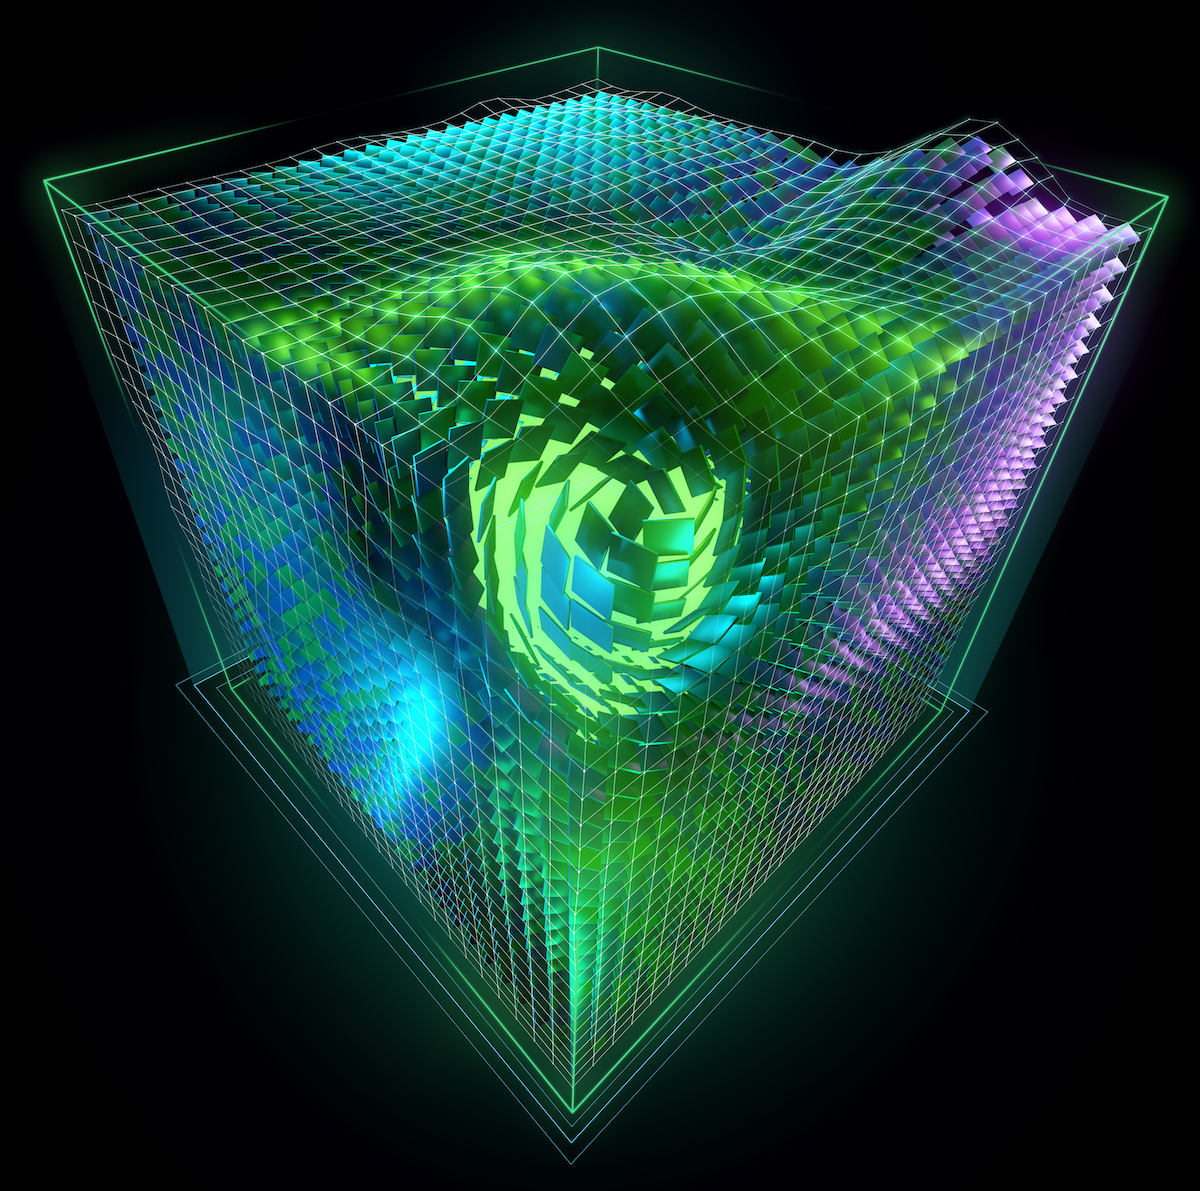
\includegraphics[scale=0.25]{./images/CUDA_Cube_1K.jpg}

\vspace{0.7cm}

Πέτρος Αγγελής, 6268 \par
\texttt{pangelis@ceid.upatras.gr}

\vspace{0.5cm}

Δαμιανός Ντούμη - Σιγάλας, 6157 \par
\texttt{nsigalas@ceid.upatras.gr}

\vspace{0.5cm}

Ανδρέας Τσαλίδης, 6239 \par
\texttt{tsalidis@ceid.upatras.gr}


\end{center}

\newpage

\lstset{basicstyle=\large,style=myCustomMatlabStyle}
\color{black}

\setlength{\parskip}{10pt}
 \pagecolor{white} 
 
 \tableofcontents
\newpage
 
\setcounter{section}{-1}
 
\section{Τεχνικά Χαρακτηριστικά}
\noindent Η εκτέλεση των προγραμμάτων μας έγινε χρησιμοποιώντας τους υπολογιστικούς πόρους που μας διετέθησαν στα πλαίσια του μαθήματος. Συγκεκριμένα η κάρτα γραφικών που αξιοποιήσαμε περιγράφεται από τα παρακάτω τεχνικά χαρακτηριστικά, με \textbf{Compute Capability 2.0}. Επιπρόσθετα η CPU που είχαμε στη διάθεση μας ήταν ενας Intel Xeon E5530 @ 2.40GHz με 8 πυρήνες και 8KB L3 cache με 12GB διαθέσιμης μνήμης RAM. Στα πλαίσια της εργασίας δεν αξιοποιείται κάποια δυνατότητα παραλληλίας στη CPU.

\begin{verbatim}
Device 0: "Tesla C2075"
  CUDA Driver Version / Runtime Version          6.0 / 6.0
  CUDA Capability Major/Minor version number:    2.0
  Total amount of global memory:                 5375 MBytes (5636554752 bytes)
  (14) Multiprocessors, ( 32) CUDA Cores/MP:     448 CUDA Cores
  GPU Clock rate:                                1147 MHz (1.15 GHz)
  Memory Clock rate:                             1566 Mhz
  Memory Bus Width:                              384-bit
  L2 Cache Size:                                 786432 bytes
  Maximum Texture Dimension Size (x,y,z)         1D=(65536), 2D=(65536, 65535), 
                                                 3D=(2048, 2048, 2048)
  Maximum Layered 1D Texture Size, (num) layers  1D=(16384), 2048 layers
  Maximum Layered 2D Texture Size, (num) layers  2D=(16384, 16384), 2048 layers
  Total amount of constant memory:               65536 bytes
  Total amount of shared memory per block:       49152 bytes
  Total number of registers available per block: 32768
  Warp size:                                     32
  Maximum number of threads per multiprocessor:  1536
  Maximum number of threads per block:           1024
  Max dimension size of a thread block (x,y,z): (1024, 1024, 64)
  Max dimension size of a grid size    (x,y,z): (65535, 65535, 65535)
  Maximum memory pitch:                          2147483647 bytes
  Texture alignment:                             512 bytes
  Concurrent copy and kernel execution:          Yes with 2 copy engine(s)
  Run time limit on kernels:                     No
  Integrated GPU sharing Host Memory:            No
  Support host page-locked memory mapping:       Yes
  Alignment requirement for Surfaces:            Yes
  Device has ECC support:                        Enabled
  Device supports Unified Addressing (UVA):      Yes
  Device PCI Bus ID / PCI location ID:           66 / 0

\end{verbatim}

Για την χρονομέτρηση των υπολογιστικών πυρήνων (kernels) χρησιμοποιούμε τα κατάλληλα cuda events που μας παρέχονται από τις βιβλιοθήκες της CUDA. Αν χρησιμοποιούσαμε κάποια λύση που βασίζεται σε βιβλιοθήκες που μας προσφέρει ο host, χωρίς την χρήση κάποιου επιπλέον ρητού συγχρονισμού θα μετράγαμε τον χρόνο εκκίνησης του υπολογιστικού πυρήνα και όχι τον χρόνο εκτέλεσής του, καθώς η εκτέλεση του kernel στην GPU είναι ασύγχρονη ως προς την υπόλοιπη ροή του προγράμματος στη CPU \cite{Harris:metrics}. Τέλος, τον παραδοτέο κώδικα συνοδεύουν κάποια απλουστευμένα Makefiles, ανεξάρτητα για κάθε ερώτημα, για την πιο εύκολη μεταγλώττισή του.

\newpage

\section{2D Convolution}
\noindent Στο πρώτο ερώτημα της εργασίας καλούμαστε να υλοποιήσουμε στη GPU την 2D συνέλιξη ενός \mbox{μητρώου A}. Για τον υπολογισμό της νέας τιμής στη θέση (i,j) χρησιμοποιείται η τιμή της τρέχουσας θέσης καθώς και οι τιμές των οχτώ γειτονικών της, κάθε μία εκ των οποίων συνεισφέρει με ένα συγκεκριμένο βάρος στο τελικό αποτέλεσμα. Στο μητρώο Β, το οποίο αποθηκεύει τις υπολογισθείσες τιμές, για τις περιφερειακές (οριακές) θέσεις του πίνακα δεν γίνεται κάποιος υπολογισμός με αποτέλεσμα να συμπληρώνονται με μηδενικά.

\begin{center}
    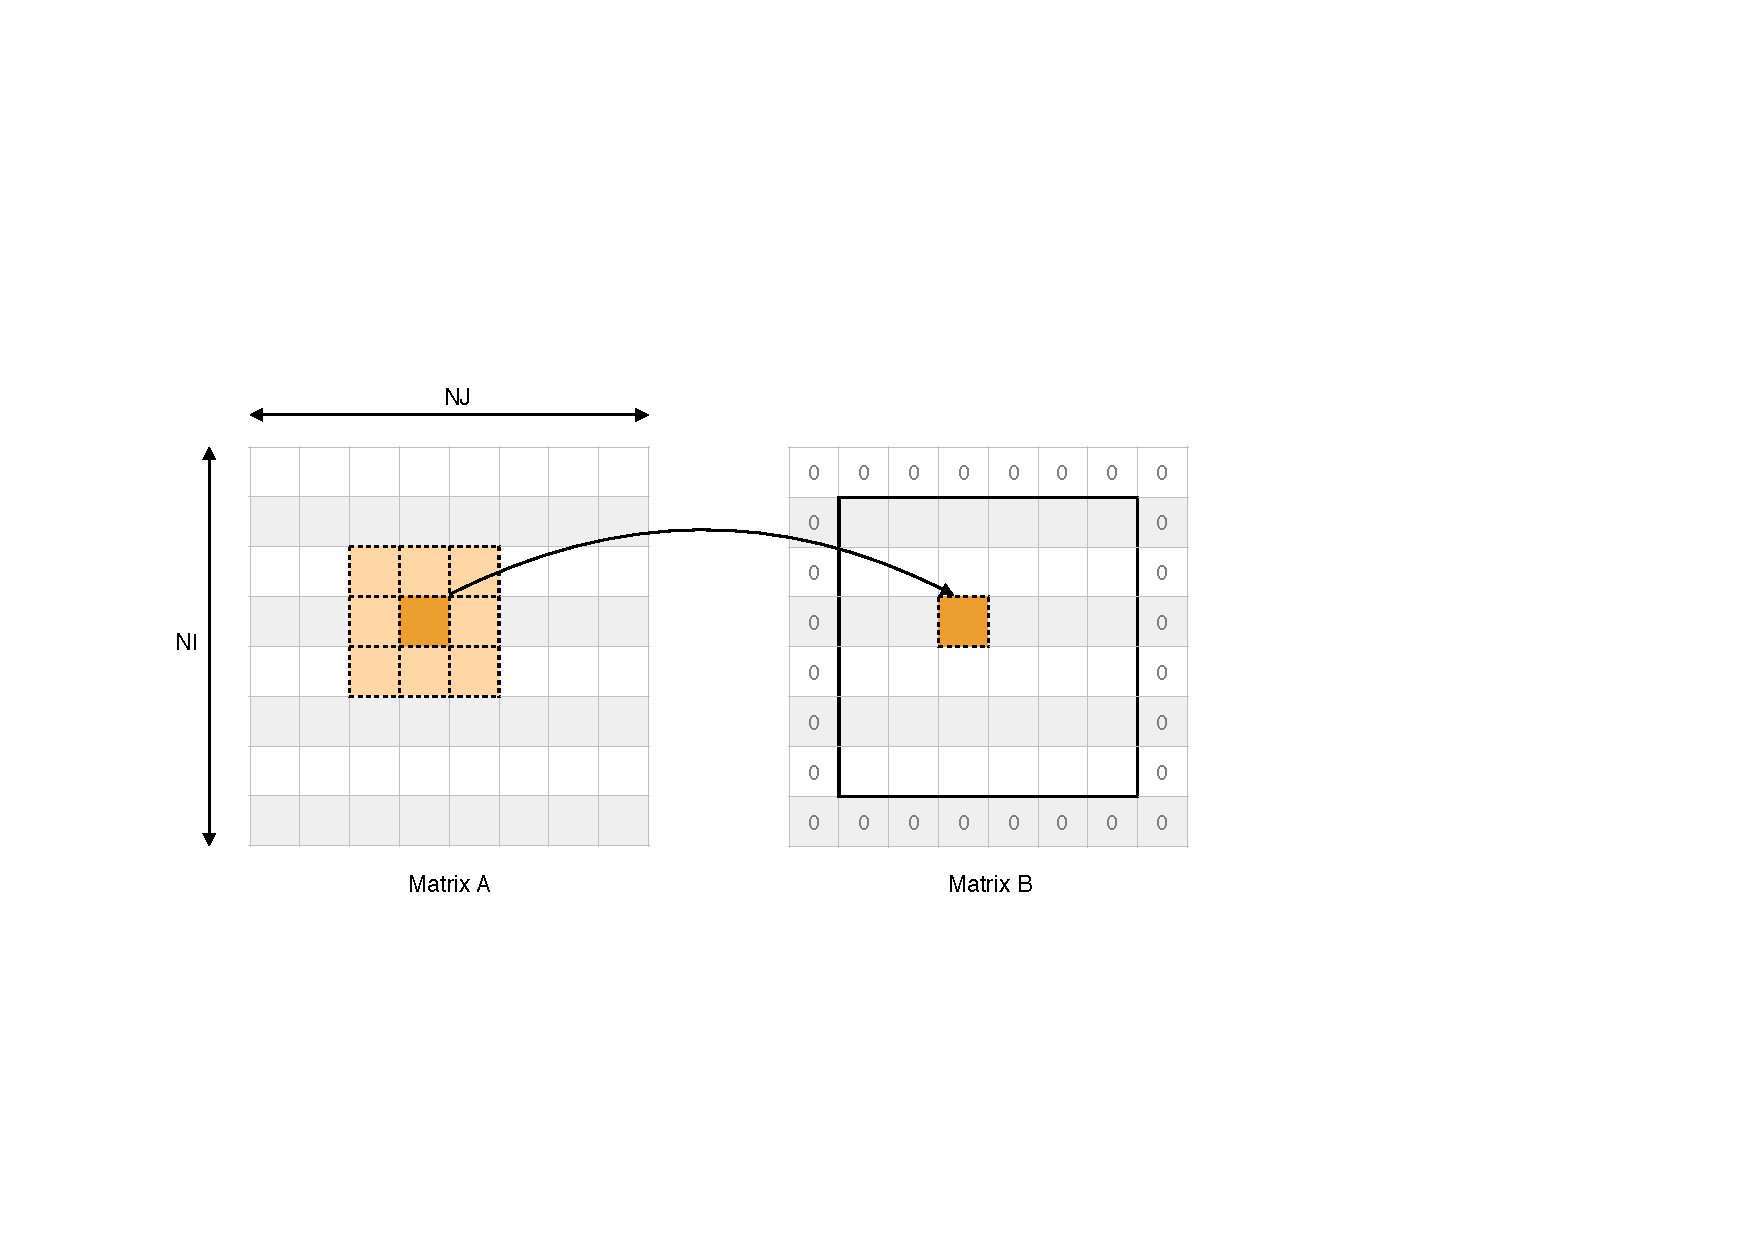
\includegraphics[scale=0.8]{./figures/1_conv/2d_conv}
\end{center}

\vspace{-0.8cm}
\subsection*{Πως όμως εξασφαλίζουμε την ορθότητα των υπολογισμών στη GPU;}
\addcontentsline{toc}{subsection}{Έλεγχος ορθότητας υπολογισμών}

Ένα ερώτημα που προκύπτει μετά την παραλληλοποίηση του κώδικα είναι αν έχει γίνει με σωστό τρόπο. Το γεγονός ότι εκτελείται χωρίς σφάλματα δεν μας εγγυάται την ορθότητα των υπολογισμών. Για την εξακρίβωσή της απαιτείται να καταστρώσουμε μια τεχνική ελέγχου η οποία θα μας διασφαλίζει ότι τελικά το μητρώο που υπολογίστηκε είναι το ζητούμενο. Σε μικρού μεγέθους προβλήματα ο οπτικός έλεγχος είναι εφικτός αφού μπορούμε να εκτυπώσουμε στην οθόνη τα αποτελέσματα και να τα αντιπαραβάλουμε με αυτά που προκύπτουν από τον αρχικό κώδικα. Με αυτόν τον τρόπο είναι πιο εύκολο να έχουμε μια πρώτη εικόνα του υπολογισμού μας η οποία μας επιτρέπει να ελέγξουμε με ευκολία τις οριακές περιπτώσεις, όπως τι συμβαίνει στα άκρα του μητρώου.

Για μεγαλύτερου μεγέθους προβλήματα αποφασίσαμε να ακολουθήσουμε μια τεχνική παρόμοια με αυτήν που παρουσιάστηκε στο μάθημα της Παράλληλης Επεξεργασίας κατά το προηγούμενο ακαδημαϊκό έτος. Συγκεκριμένα διατρέχουμε το μητρώο και αποθηκεύουμε είτε δειγματοληπτικά είτε το σύνολο των τιμών (όταν το μέγεθός του μας το επιτρέπει) σε ένα αρχείο. Κάνουμε το ίδιο και για τον αρχικό κώδικα και έπειτα τα συγκρίνουμε τα δύο αρχεία με χρήση της \texttt{numdiff}. Θεωρούμε ότι οι υπολογισμοί μας είναι ορθοί όταν οι τιμές που περιέχουν είναι ίσες (λαμβάνοντας υπόψιν ένα άνω όριο απόλυτου σφάλματος).

\vspace{-0.3cm}

\subsection*{Επιλογή μεγέθους block και grid}
\addcontentsline{toc}{subsection}{Επιλογή μεγέθους block και grid}

Το επόμενο θέμα που μας απασχόλησε είναι ποια είναι τα βέλτιστα μεγέθη block και grid για τα οποία παίρνουμε την καλύτερη απόδοση; Αφού το πρόβλημα μας περιέχει μητρώα δύο διαστάσεων, θα χρησιμοποιήσουμε δισδιάστατα block και grid. Τι μέγεθος όμως θα ορίσουμε σε κάθε μία από τις διαστάσεις για καθένα από αυτά τα δύο στοιχεία; Κάποια στοιχεία που πρέπει να ληφθούν υπόψιν περιγράφονται παρακάτω:

\begin{itemize}
    \item Το μέγεθος κάθε block δεν πρέπει να ξεπερνά τα 1024 threads με μέγιστες διαστάσεις (1024, 1024, 64).
    \item Κάθε block δεν μπορεί να καταναλώνει περισσότερους από 32k καταχωρητές.
    \item Κάθε block δεν μπορεί να καταναλώνει περισσότερο από 48kb shared memory.
    \item Ιδανικά, ο αριθμός των thread ανα block πρέπει να είναι πολλαπλάσιο του warp size (32 threads).
    H Tesla C2075 έχει 1.536 thread slots per SM. Αφού 1.536 = 32 × 48, έχουμε \#thread slots = warp size × \#warps per block. Αν έχω 32 threads ανα block, 1.536 / 32 = 48 blocks / SM το μέγιστο.
    
    \item Κάθε SM της GPU ιδανικά πρέπει να έχει αρκετά ενεργά warps ώστε να προσεγγίζουμε την μέγιστη διεκπεραιωτική ικανότητα (throughput).
\end{itemize}

Γίνεται φανερό ότι δεν υπάρχει ένας ντετερμινιστικός τρόπος να καθορίσουμε το ιδανικό μέγεθος block και grid αφού αυτά εξαρτώνται τόσο από περιορισμούς στο hardware που θέτει η εκάστοτε κάρτα όσο και στην φύση του κώδικα μας. Για τον λόγο αυτό έχοντας υπόψιν τις παραπάνω παραμέτρους πειραματιζόμαστε δοκιμάζοντας διαφορετικούς συνδυασμούς από τον ``χώρο αναζήτησης'' μας μέχρι να βρούμε για ποια μεγέθη το πρόγραμμα μας συμπεριφέρεται με ικανοποιητικό τρόπο. Παρακάτω παρατίθενται κάποιες ενδεικτικές μετρήσεις από την διαδικασία αυτή οι οποίες επιβεβαιώνουν την διαίσθηση μας.

\vspace{-0.3cm}
\subsection*{Αποτελέσματα}
\addcontentsline{toc}{subsection}{Αποτελέσματα}

\begin{center}
    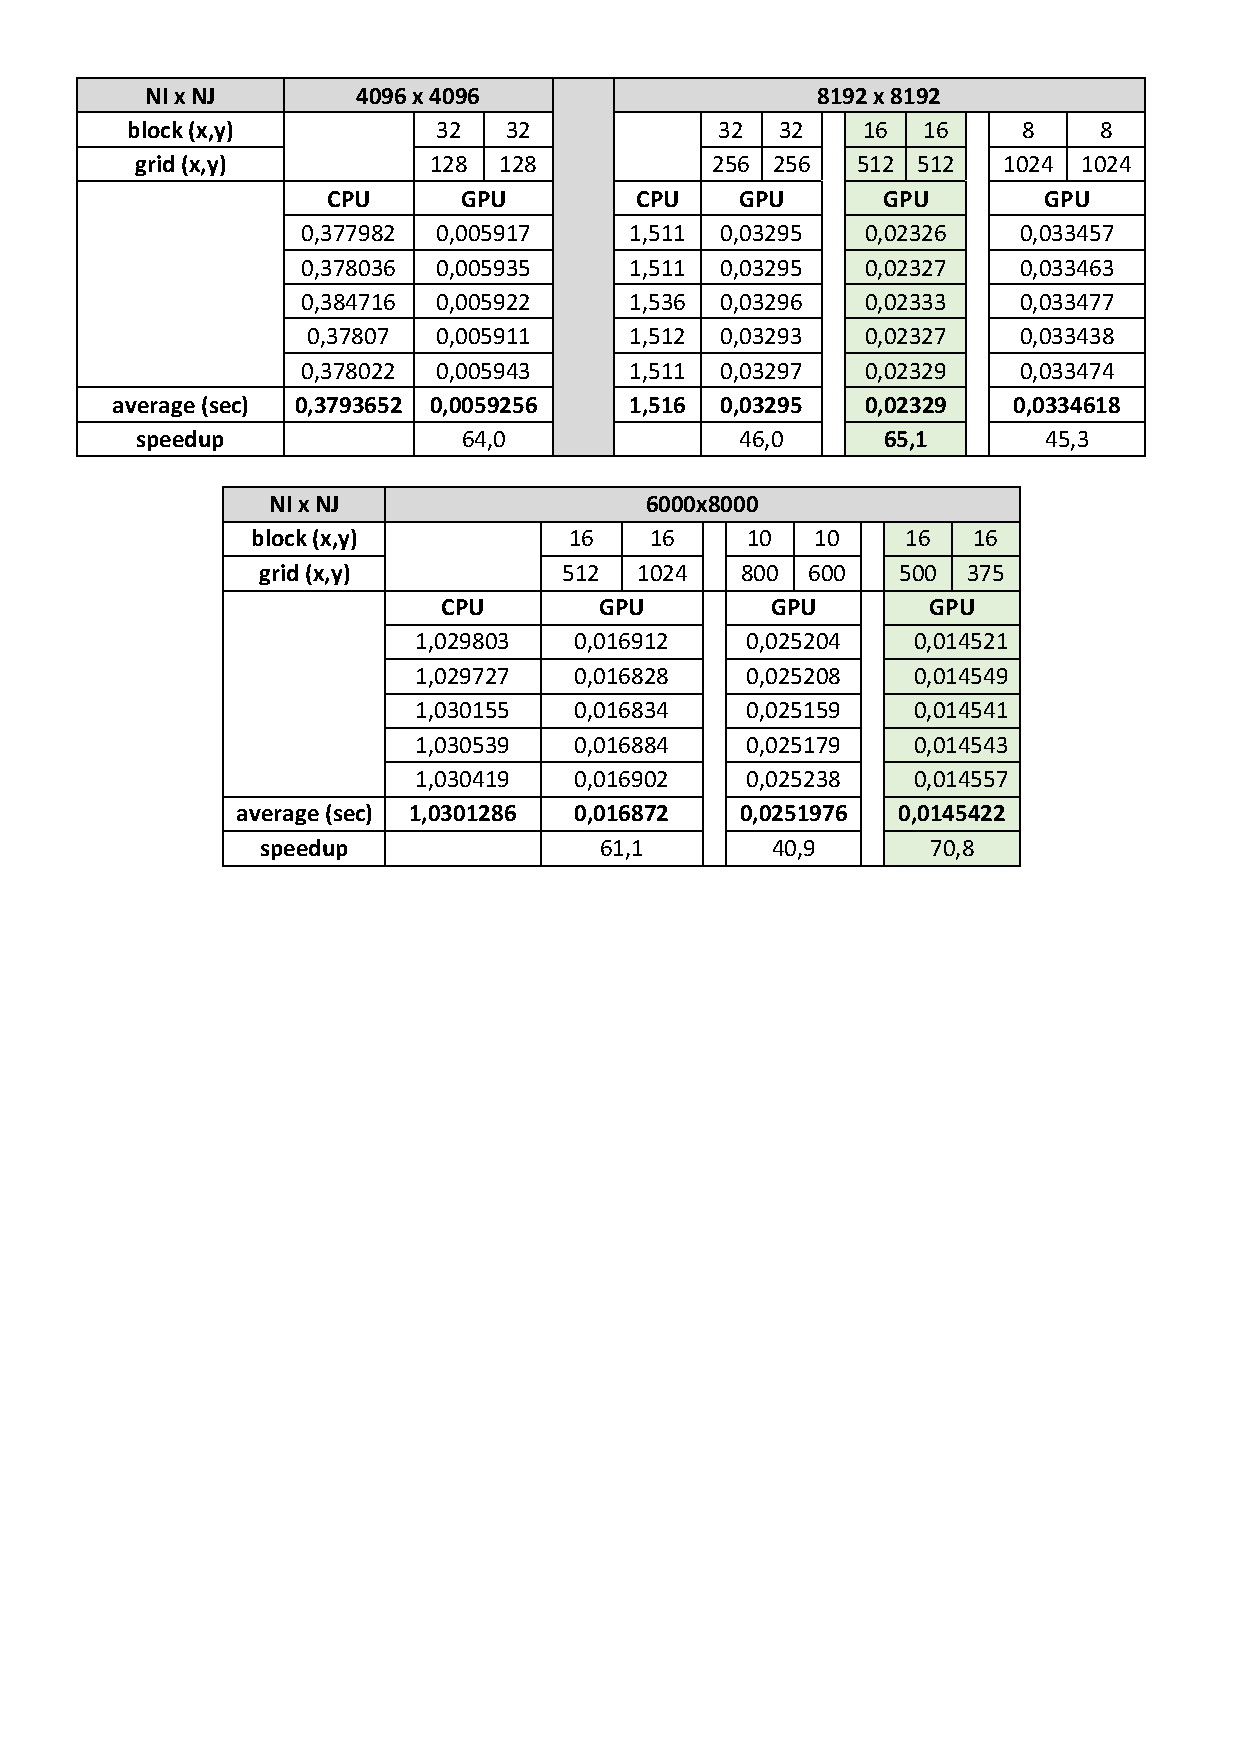
\includegraphics[scale=0.8]{./figures/1_conv/table1}
\end{center}

Ιδιαίτερο ενδιαφέρον παρουσιάζει η περίπτωση στην οποία το μέγεθος του μητρώου είναι 6000Χ8000, ένα grid αρκετά μεγαλύτερο από το μητρώο δίνει σημαντικά καλύτερη απόδοση από ένα άλλο grid με διαστάσεις που ενώ  ταιριάζουν ακριβώς στο αρχικό μητρώο, δεν έχουν μέγεθος block πολλαπλάσιο του warp size. Σε κάθε περίπτωση καλύτερη απόδοση επιτυγχάνουμε όταν για 16×16 block χρησιμοποιούμε το μικρότερο δυνατό grid. Αφού λοιπόν καταλήξαμε ότι στις περισσότερες περιπτώσεις block μεγέθους 16×16 μας δίνουν την καλύτερη συμπεριφορά μπορούμε να εκφράσουμε αλγοριθμικά τον υπολογισμό του απαιτούμενου μεγέθους για το grid ανάλογα με το μέγεθος της εισόδου (NI, NJ) ως εξής:

\vspace{0.3cm}

\newpage

\begin{lstlisting}[language=C]
    // given block size
	int block_dim_x = 16;
	int block_dim_y = 16;

	// calculate grid dimensions
	int grid_dim_x = ceil( (float) NJ / block_dim_x );
	int grid_dim_y = ceil( (float) NI / block_dim_y );
\end{lstlisting}

\begin{center}
    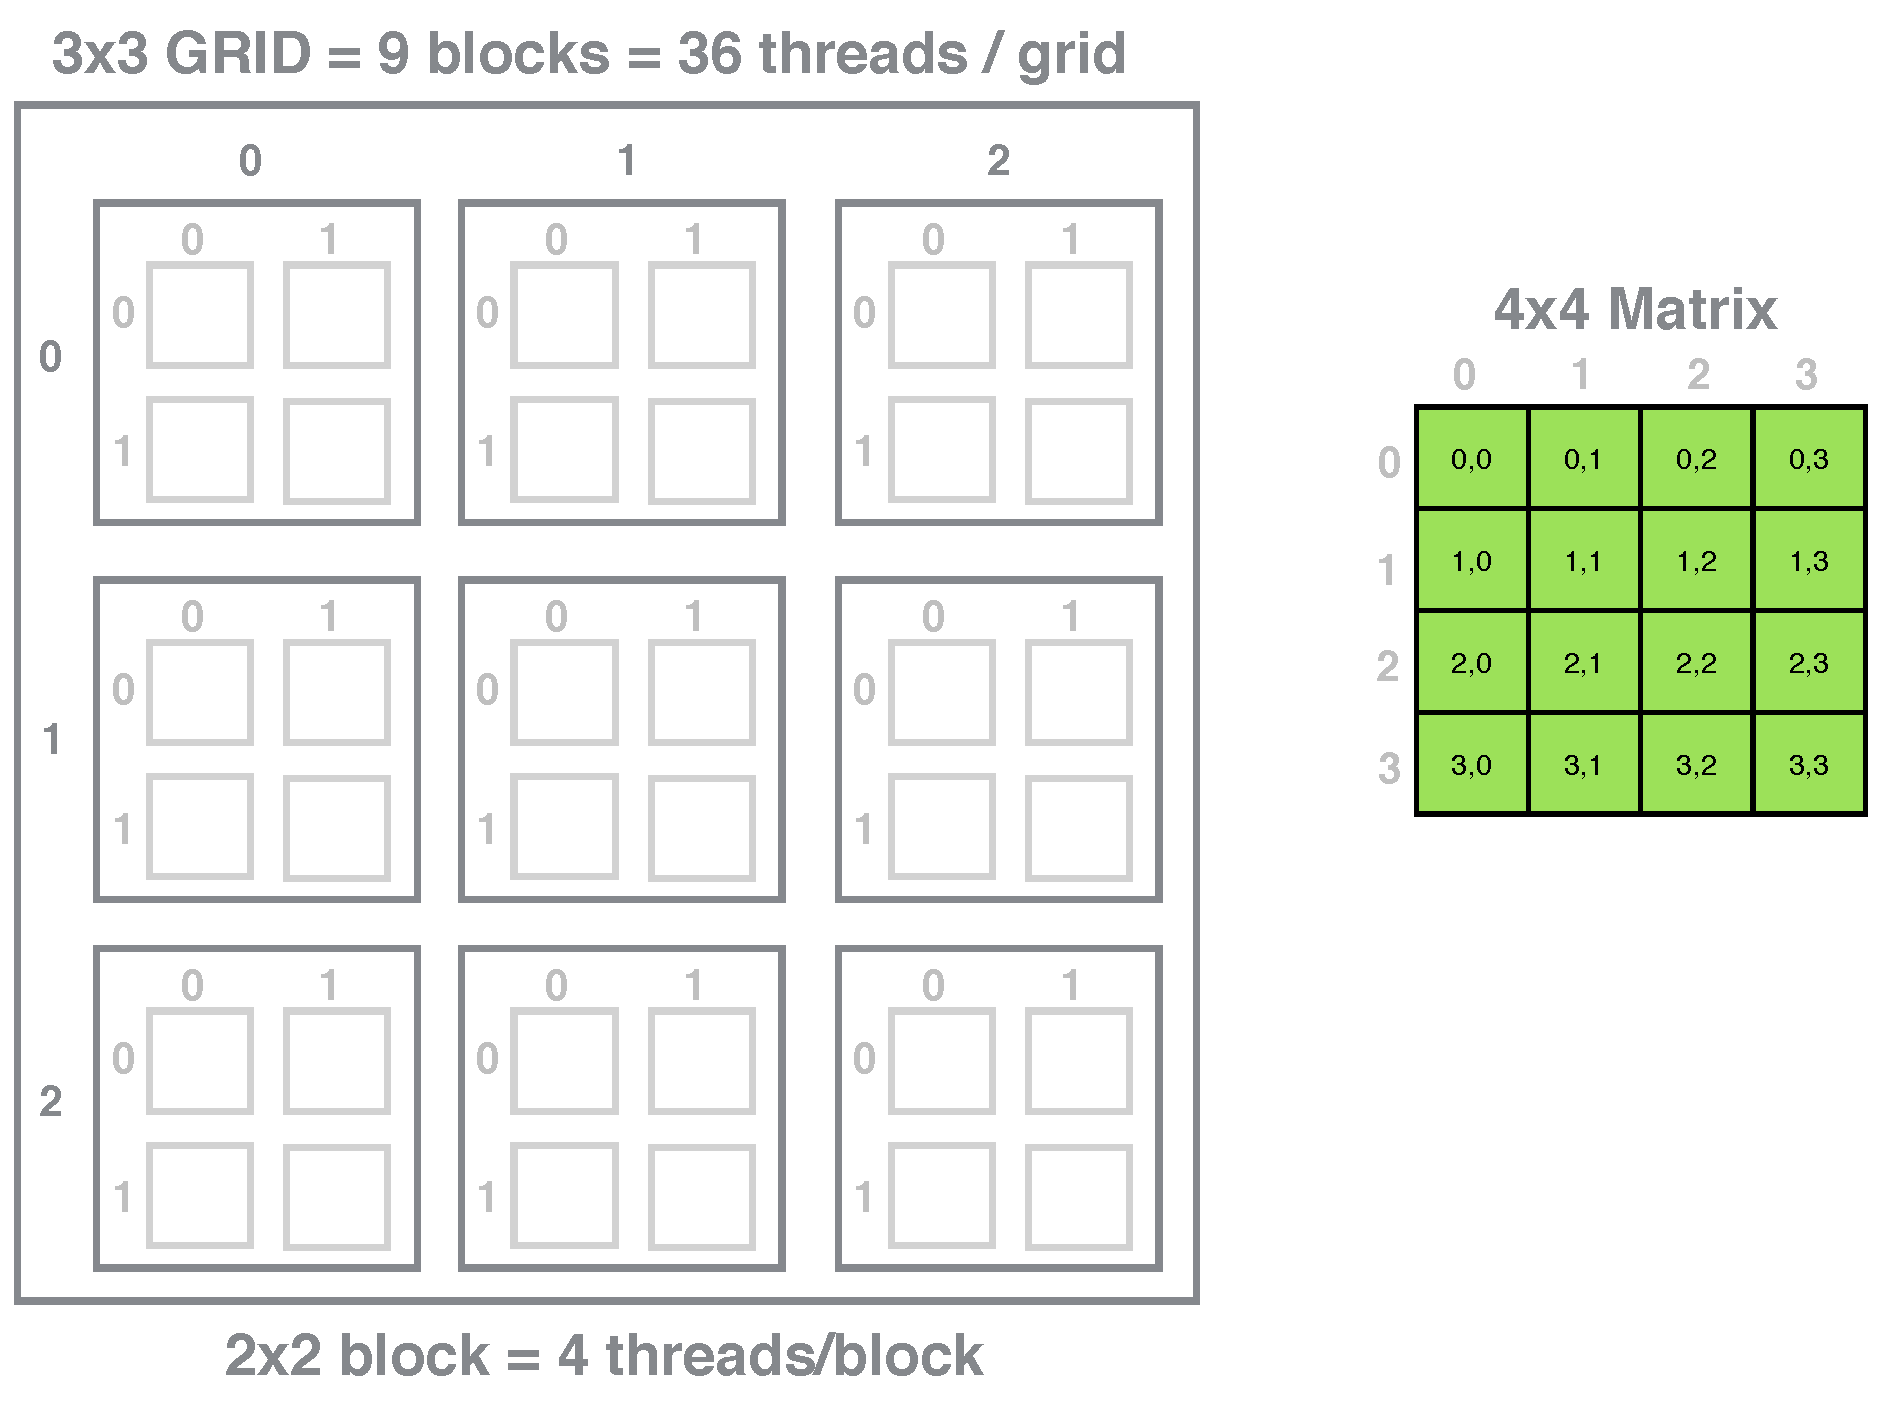
\includegraphics[scale=0.35]{./figures/1_conv/grid-matrix}
\end{center}

\begin{center}
    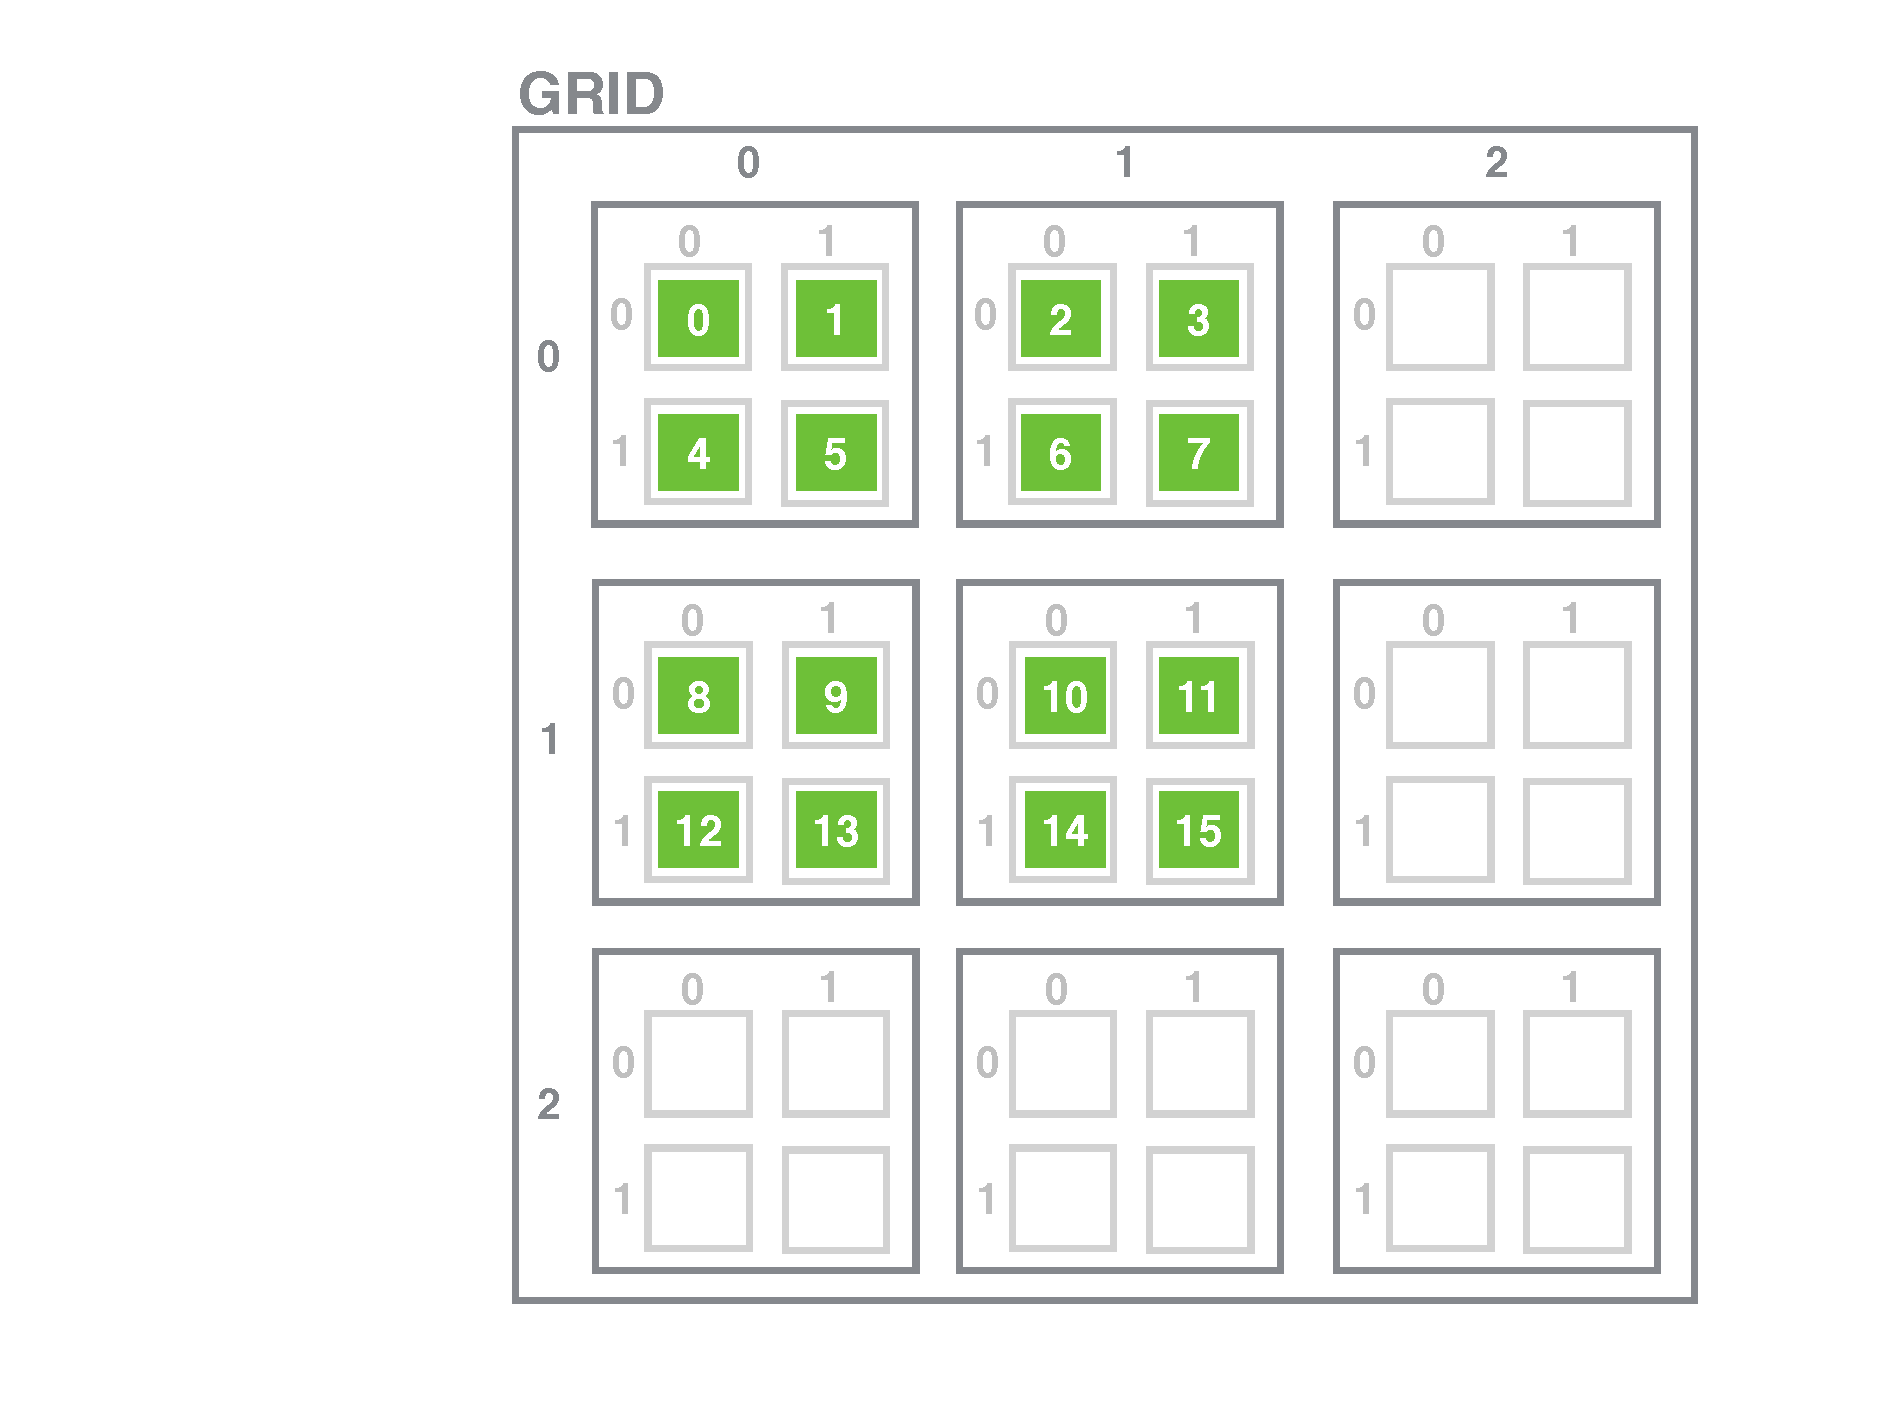
\includegraphics[scale=0.35]{./figures/1_conv/final-grid}
\end{center}

Στο παραπάνω σχήμα φαίνεται ο τρόπος με τον οποίο αντιστοιχούμε ένα 4x4 μητρώο σε δεδομένων διαστάσεων grid, μέσω της μονοδιάστατης αναπαράστασής του στην μνήμη. Στην πραγματικότητα βέβαια τα πράγματα είναι διαφορετικά αφού δεν χρησιμοποιούμε προκαθορισμένες διαστάσεις για το grid αλλά ο αριθμός των block καθορίζεται δυναμικά ώστε να είναι ο ελάχιστος απαραίτητος σε κάθε διάσταση.

\newpage

\section{y = A\textsuperscript{T} {$\cdot$} A {$\cdot$} x}
%\setlength{\parindent}{0pt}

\noindent Στο ζητούμενο αυτό καλούμαστε να υλοποιήσουμε στη GPU την παρακάτω πράξη:

\vspace{-0.5cm}
$$ y = A^{T} \cdot A \cdot x$$

\noindent όπου:\\
\textbf{Α}: μητρώο διαστάσεων NX × NY,\\
\textbf{x}: διάνυσμα (διαστάσεων NY × 1),\\
\textbf{Α\textsuperscript{T}}: ανάστροφο του A (NΥ × NΧ) και\\
\textbf{y}: το ζητούμενο διάνυσμα διαστάσεων NY × 1

Στην δοθείσα σειριακή εκδοχή παρατηρούμε ότι ο υπολογισμός του αποτελέσματος γίνεται σταδιακά σε έναν βρόγχο for όπου σε κάθε βήμα υπολογίζεται το εσωτερικό/στικτό γινόμενο (dot product) της τρέχουσας γραμμής που βρίσκεται ο υπολογισμός και στην συνέχεια με βάση αυτό ενημερώνεται το διάνυσμα y, κάνοντας ουσιαστικά την αντίστοιχη διαδικασία.

\noindent Για να μεταφέρουμε την λειτουργία αυτή σε CUDA αξιοποιώντας λειτουργίες όπως η shared memory, προχωρήσαμε στην αναδιοργάνωση των υπολογισμών ως εξής:

\vspace{-0.4cm}
$$ \Big( A^{T} \cdot ( A \cdot x ) \Big) = y$$

Αρχικά προκειμένου να γλυτώσουμε υπολογισμούς πρώτη γίνεται η πράξη $( A \cdot x )$ από την οποία προκύπτει ένα διάνυσμα-στήλη μεγέθους NX στοιχείων. Έπειτα πολλαπλασιάζεται ο ανάστροφος $A^{T}$ με το διάνυσμα που υπολογίστηκε στο προηγούμενο βήμα. Έτσι προκύπτει το ζητούμενο διάνυσμα y μεγέθους NY στοιχείων. Στο σημείο αυτό τίθενται δύο κύριοι προβληματισμοί μας σχετικά με το πώς θα αντιμετωπίσουμε την διαδικασία αυτή. Ο πρώτος είναι ότι επειδή θα έχουμε ήδη μεταφέρει το μητρώο A στην μνήμη της GPU θα πρέπει να το εκμεταλλευτούμε τόσο ως το κανονικό όσο ως και το ανάστροφό του. Ακόμα και αν κάναμε την αναστροφή του στην GPU πέρα από σπατάλη χρόνου θα είχαμε και σπατάλη χώρου, ο οποίος όσο μεγαλώνει το μέγεθος της εισόδου γίνεται όλο και πιο περιορισμένος. Το δεύτερο σημείο που μας απασχόλησε αφορά ποιες δυνατότητες και με ποιον τρόπο θα τις χρησιμοποιήσουμε ώστε να αξιοποιήσουμε τα πλεονεκτήματα του παράλληλου υπολογισμού που μας προσφέρει η κάρτα γραφικών.

\subsection*{Μητρώο Α και ανάστροφο Α\textsuperscript{T}}
\addcontentsline{toc}{subsection}{Μητρώο Α και ανάστροφο Α\textsuperscript{T}}

\noindent Για τον υπολογισμό του αποτελέσματος χρειάζεται να διατρέξουμε τόσο το μητρώο Α όσο και το ανάστροφό του. Ο τρόπος με τον οποίο αρχικοποιούμε το Α αντιστοιχεί στην κατά-γραμμές (row-major) αναπαράσταση του στην μνήμη όπου διαδοχικές γραμμές αποθηκεύονται σε διαδοχικές θέσεις μνήμης όπως φαίνεται και στο σχήμα παρακάτω.

\begin{center}
    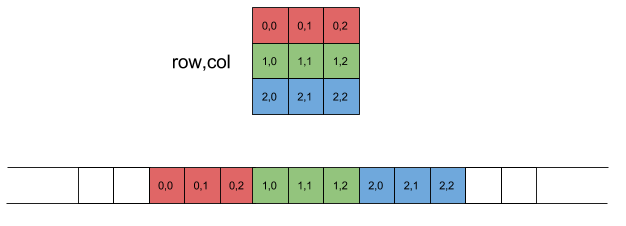
\includegraphics[scale=0.6]{./figures/2_tnv/row-major-2D}
\end{center}

\newpage \noindent Αντίθετα μία κατά στήλες (column-major) αναπαράσταση του μητρώου στην μνήμη θα ήταν η αντίστοιχη: 

\begin{center}
    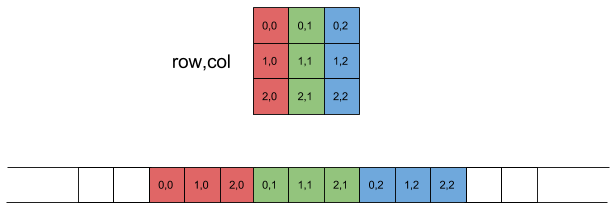
\includegraphics[scale=0.6]{./figures/2_tnv/column-major-2D}
\end{center} 

Σε κάθε περίπτωση εμείς στην υλοποίησή μας διαθέτουμε τα δεδομένα μας στην εξής μορφή:

\begin{center}
    Matrix A = 
\begin{pmatrix} 
0 & 1 & 2 \\
3 & 4 & 5 \\
6 & 7 & 8
\end{pmatrix}
\hspace{0.5cm}Matrix A\textsuperscript{T} =
\begin{pmatrix} 
0 & 3 & 6 \\
1 & 4 & 7 \\
2 & 5 & 8
\end{pmatrix}

\vspace{0.4cm}

{\large \texttt{A[] = \{0, 1, 2, 3, 4, 5, 6, 7, 8\}}}

\end{center}

Έτσι λοιπόν προκειμένου να αποφύγουμε την διπλή αποθήκευση του μητρώου στην μνήμη, εκμεταλλευόμαστε την παρουσία του Α ώστε διατρέχοντας το με τον κατάλληλο τρόπο να προσπευλαύνουμε το ανάστροφό του. Η πρακτική αυτή συνδέεται στενά με την έννοια του coalescing που περιγράφεται παρακάτω.



\subsection*{Memory Coalescing / Row-Major \& Column-Major Traversal}
\addcontentsline{toc}{subsection}{Memory Coalescing / Row-Major \& Column-Major Traversal}


\begin{center}
    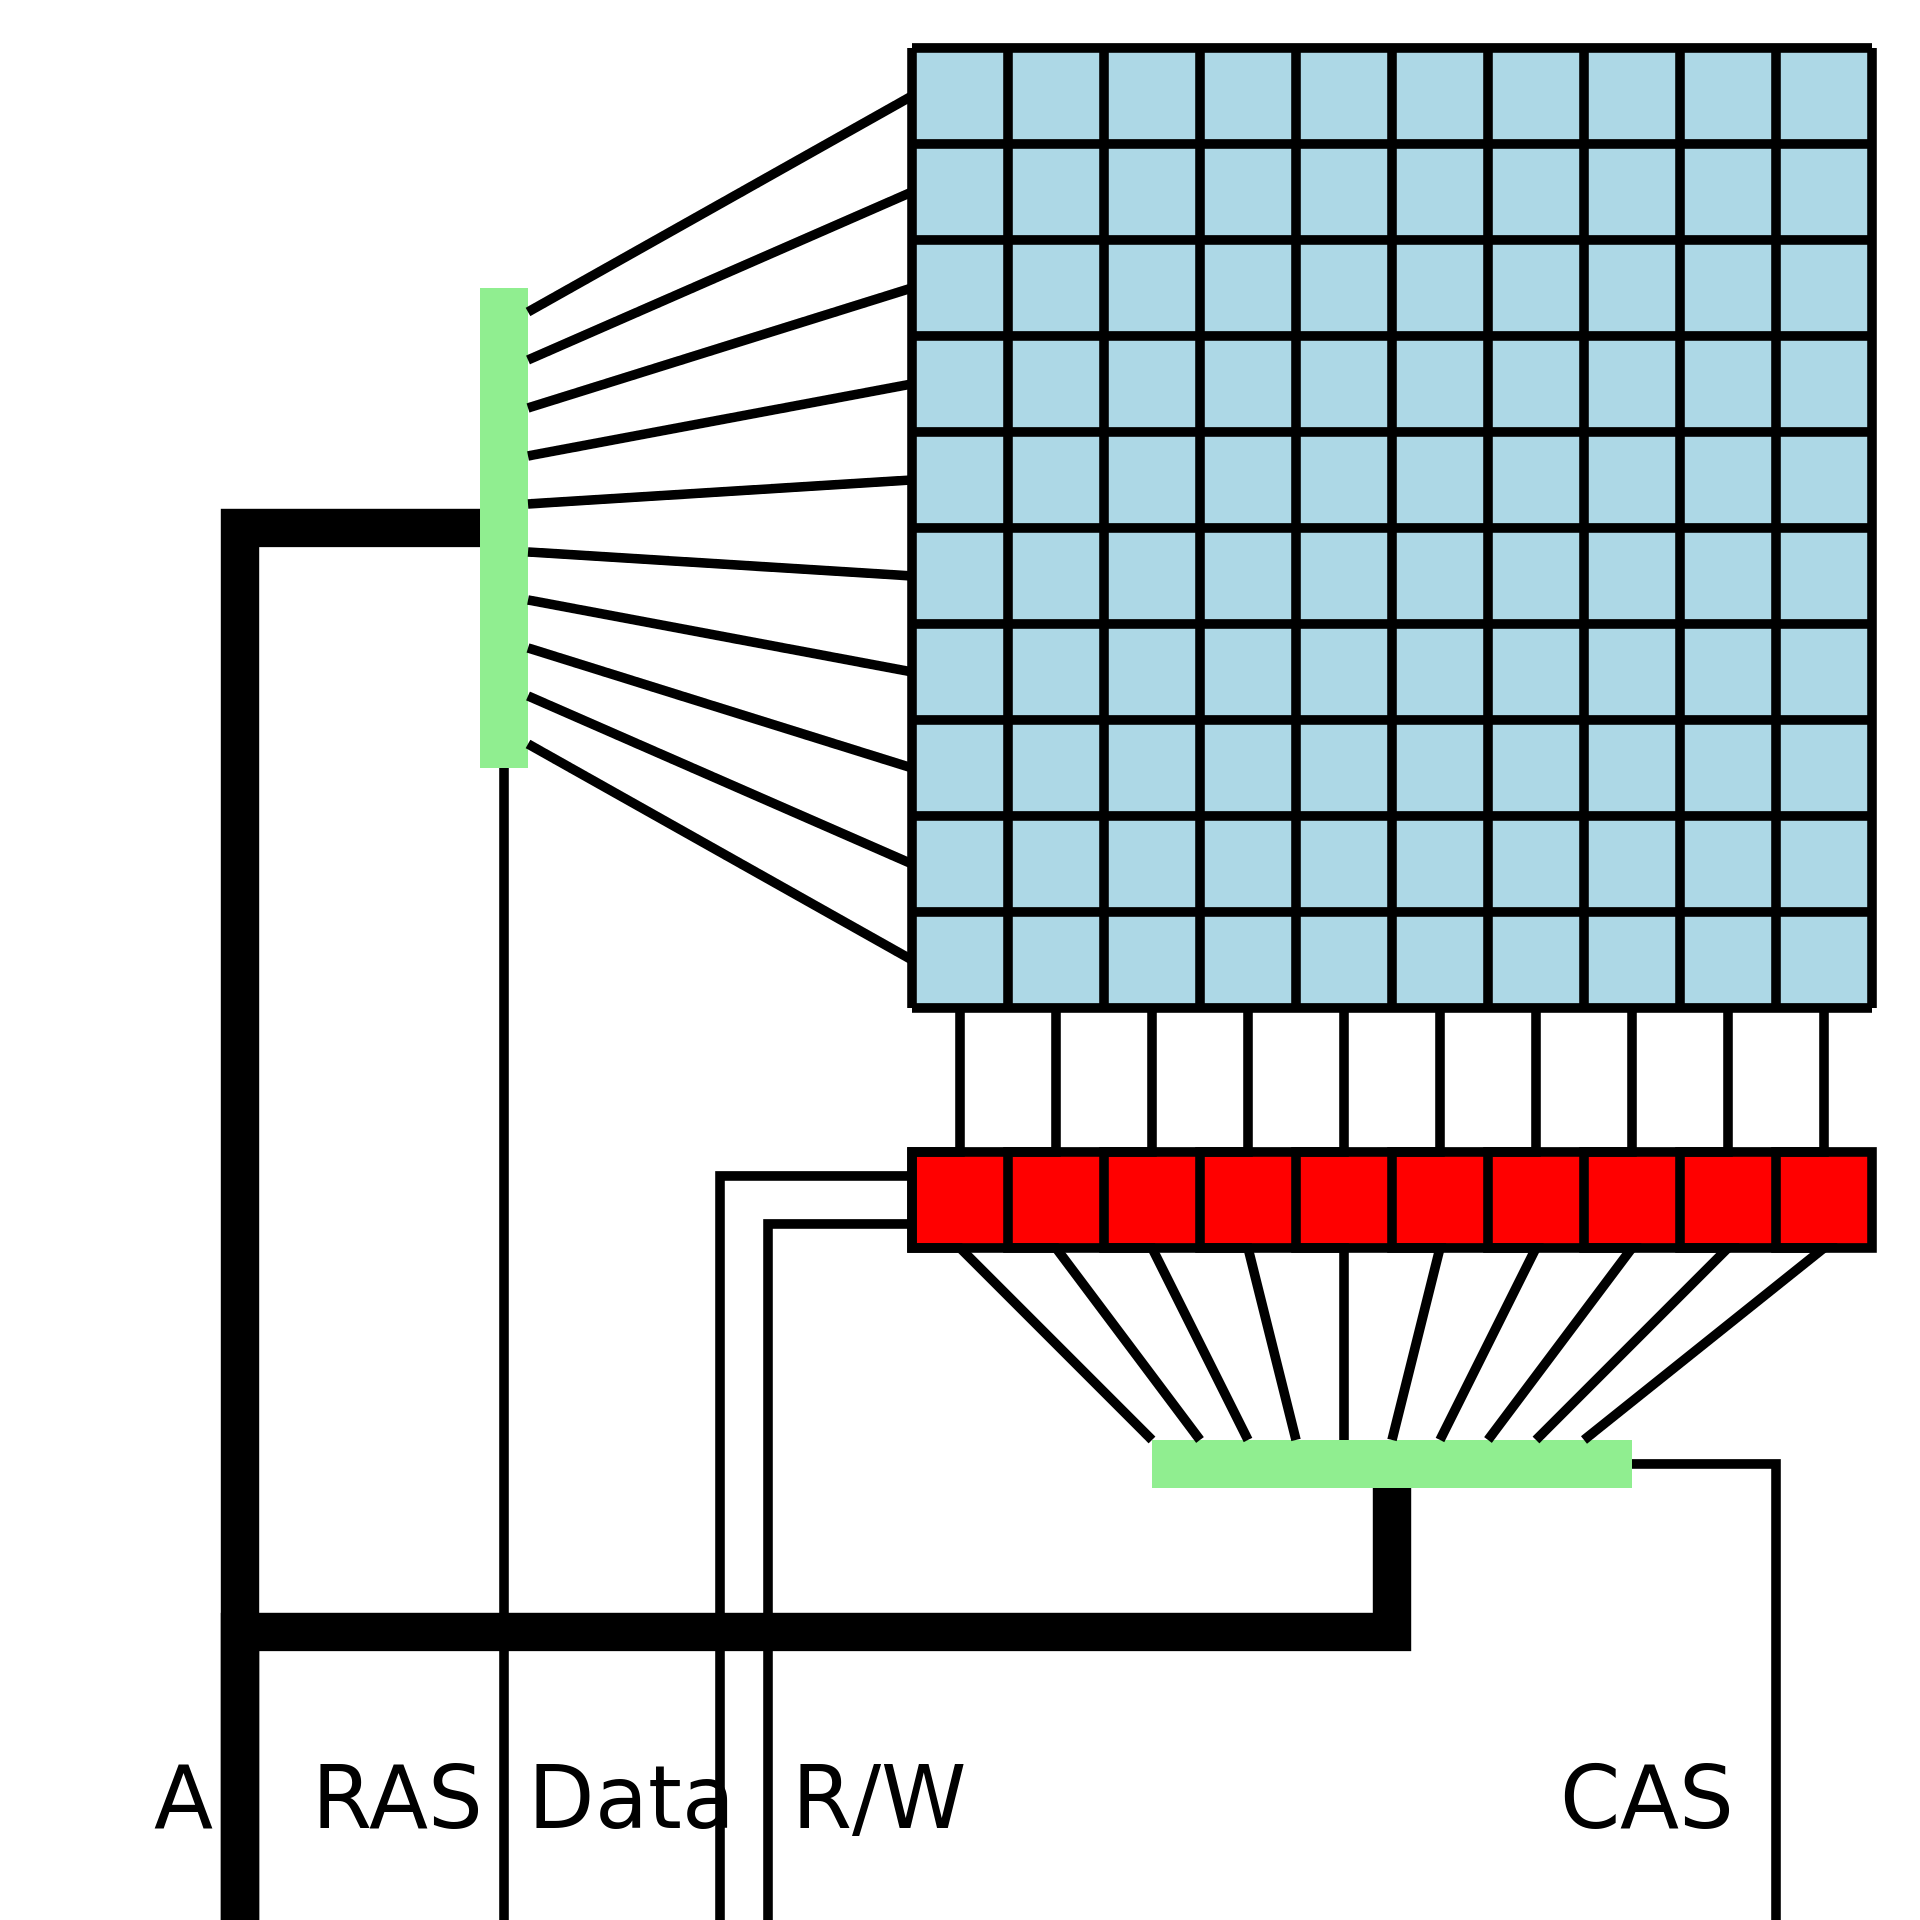
\includegraphics[scale=0.1]{./figures/2_tnv/DRAM}
    
    {\small \textit{Τυπική αρχιτεκτονική DRAM bank}}
\end{center}

Εξ αιτίας της κατασκευής των DRAM, όπου ο τρισδιάστατος, οργανωμένος σε banks φυσικός χώρος διευθύνσεων, αντιστοιχίζεται σε έναν γραμμικό λογικό χώρο, όταν προσπελαύνεται μία θέση μνήμης στην πραγματικότητα γίνονται διαθέσιμα τα δεδομένα περισσότερων από μία διαδοχικών διευθύνσεων.
Λαμβάνοντας υπόψιν ότι όλα τα thread σε ένα warp εκτελούν την ίδια εντολή, αν οργανώσουμε τον κώδικα μας με τέτοιο τρόπο ώστε τα threads κάθε χρονική στιγμή να προσπελαύνουν συνεχόμενες θέσεις μνήμης τότε εκμεταλλευόμενοι την παραπάνω συμπεριφορά μπορούμε να πετύχουμε σημαντική βελτίωση της επίδοσης του προγράμματός μας. Η τεχνική αυτή ονομάζεται memory coalescing \cite{Harris:coal}. Ας εξετάσουμε το παρακάτω παράδειγμα:


\begin{verbatim}
2D array:                   1D mapping in memory:
0  1  2  3                  0 1 2 3 4 5 6 7 8 9 a b
4  5  6  7                  element (r,c) maps to (r*4+c)
8  9  a  b

row-major traversal:                        column-major traversal:
thread 0:  0, 1, 2                          thread 0:  0, 4, 8
thread 1:  3, 4, 5                          thread 1:  1, 5, 9
thread 2:  6, 7, 8                          thread 2:  2, 6, a
thread 3:  9, a, b                          thread 3:  3, 7, b
----------time---------->                   ----------time---------->
\end{verbatim}

Θεωρούμε ότι έχουμε ένα 3Χ4 μητρώο αποθηκευμένο στην μνήμη σειριακά, με οργάνωση κατά γραμμή. Αν επίσης διαθέτουμε 4 thread καθένα εκ των οποίο σε κάθε βήμα προσπελαύνει μία θέση του πίνακα, τότε κάθε thread θα αναλάβει συνολικά την επεξεργασία τριών στοιχείων. Αν λοιπόν σε κάθε thread αντιστοιχήσουμε τα στοιχεία που του αναλογούν με έναν row-major τρόπο τότε κάθε χρονική στιγμή θα καταλήξουν να μην προσπελαύνουν διαδοχικές θέσεις μνήμης. Αντίθετα αν κάθε thread κινείται στα στοιχεία μιας στήλης (column-major traversal) τότε θα πετύχουμε το επιθυμητό αποτέλεσμα. Η συμπεριφορά αυτή γίνεται πιο εύκολα κατανοητή παρατηρώντας το παρακάτω σχήμα στο οποίο αριστερα απεικονίζονται οι θέσεις μνήμης που προσπελαύνουν τα 4 threads, στο πρώτο βήμα του υπολογισμού, αν χρησιμοποιείται row-major traversal ενω δεξιά η αντίστοιχη συμπεριφορά για column-major traversal.

%\begin{center}
    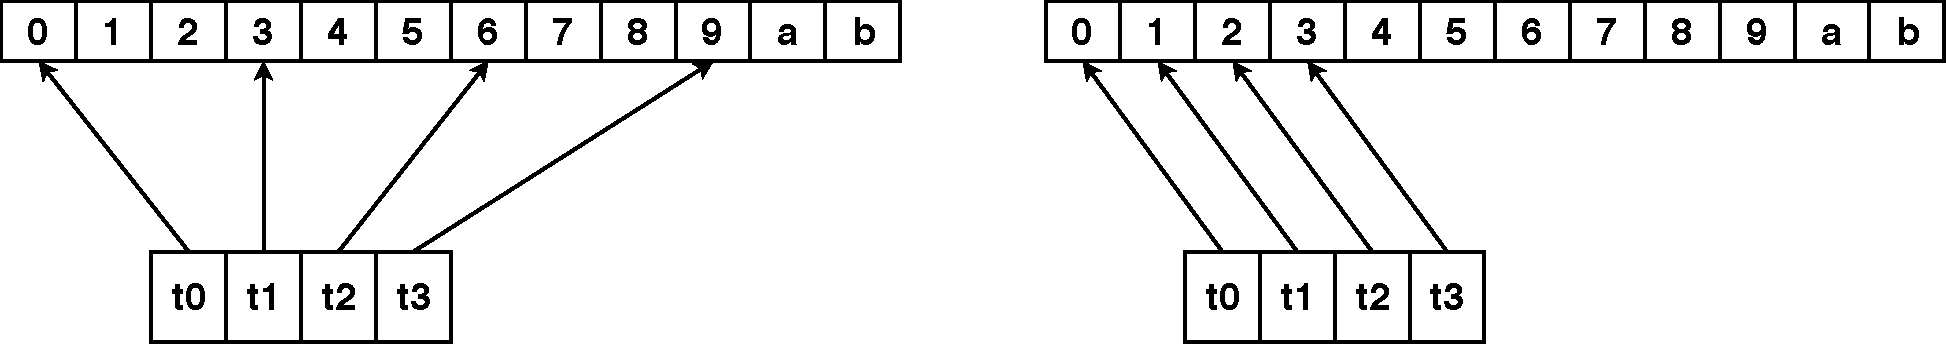
\includegraphics[scale=0.45]{./figures/2_tnv/coal.pdf}
%\end{center}

Η αξιοποίηση αυτής της τεχνικής βρίσκει άμεση εφαρμογή στο πρόβλημά μας κατά τον πολλαπλασιασμό του μητρώου A\textsuperscript{T} με το διάνυσμα (Ax). Εξαιτίας του τρόπου με τον οποίο έχουμε αποθηκευμένο το μητρώο στην μνήμη, διατρέχοντας τα στοιχεία του Α υποθέτοντας οργάνωση κατά στήλες ουσιαστικά επιτυγχάνουμε την προσπέλαση του ανάστροφού του με coalesced τρόπο. 

\subsection*{Shared Memory}
\addcontentsline{toc}{subsection}{Shared Memory}

\noindent Η προσπέλαση της shared memory είναι αρκετές τάξεις μεγέθους ταχύτερη σε σχέση με αυτήν της global memory επομένως μπορούμε να την αξιοποιήσουμε για να βελτιώσουμε την απόδοση της εφαρμογής μας. Βέβαια με τη χρήση της προκύπτουν δύο ζητήματα που πρέπει να λάβουμε υπόψιν. Αρχικά πρέπει να μεταφέρουμε στην κοινόχρηστη μνήμη μόνο τα δεδομένα που θα χρησιμοποιηθούν παραπάνω από μία φορές (ιδανικά πολλές περισσότερες) καθώς και να τροποποιήσουμε τον αλγόριθμό μας ώστε να τα χρησιμοποιεί σε μία φάση ώστε να αποφύγουμε τις εναλλασσόμενες μεταφορές των ίδιων στοιχείων. Σε περίπτωση που ένα στοιχείο χρησιμοποιείται μόνο μία φορά είναι ανώφελο να το μεταφέρουμε στην shared memory καθώς στην πράξη θα προσθέσουμε επιπλέον επιβάρυνση για τη μεταφορά και τη χρήση του.

Επίσης η shared memory είναι διαθέσιμη σε επίπεδο block. Δηλαδή μόνο τα threads του ίδιου block έχουν πρόσβαση στα κοινά δεδομένα. Το δεύτερο ζήτημα που προκύπτει είναι ότι κάθε block έχει διαθέσιμα \mbox{49152 bytes} (48KB) κοινόχρηστης μνήμης με αποτέλεσμα να πρέπει να είμαστε προσεκτικοί να μην ξεπεράσουμε το όριο αυτό. Στον δικό μας αλγόριθμο εφαρμόζουμε τη χρήση της shared memory κατά τον πολλαπλασιασμό μητρώου διανύσματος.

\newpage

\subsection*{Σύνοψη υλοποίησης}
\addcontentsline{toc}{subsection}{Σύνοψη υλοποίησης}

Η υλοποίηση μας αποτελείται από δύο υπολογιστικούς πυρήνες (kernels):
\begin{enumerate}
    \item \textbf{\texttt{\textunderscore\textunderscore global\textunderscore\textunderscore\ void matvec\textunderscore kernel\textunderscore row\textunderscore major(...)}}
    
    Στον kernel αυτόν υλοποιείται η πράξη του πολλαπλασιασμού μητρώου διανύσματος και χρησιμοποιείται για την εκτέλεση της πρώτης πράξης, δηλαδή της $(Ax)$. Για την προσπέλαση των στοιχείων του διανύσματος x γίνεται χρήση της shared memory καθώς τα στοιχεία του χρησιμοποιούνται με μεγαλύτερη συχνότητα και επαναλαμβανόμενα για τον υπολογισμού του αποτελέσματος. Το μητρώο Α βρίσκεται αποθηκευμένο στην global memory και κάθε thread πραγματοποιεί προσπέλαση στοιχείων με row-major τρόπο (υποθέτοντας οργάνωση στη μνήμη κατά γραμμές), με αποτέλεσμα οι προσπελάσεις της global memory να μην ειναι coalesced.
    
    Για την κλήση του υπολογιστικού πυρήνα έχει δημιουργηθεί μία συνάρτηση-wrapper η οποία αναλαμβάνει να υπολογίσει το απαιτούμενο grid size ανάλογα το μέγεθος του προβλήματος, την κλήση του kernel καθώς και την χρονομέτρησή του. Η συνάρτηση αυτή είναι η: \textbf{\texttt{\textunderscore\textunderscore host\textunderscore\textunderscore\  float matvec\textunderscore ROW\textunderscore MAJOR(...)}}
    
    
    
     %\newpage
     
     
    \item \textbf{\texttt{\textunderscore\textunderscore global\textunderscore\textunderscore\ void matvec\textunderscore kernel\textunderscore column\textunderscore major(...)}}
    
    Στον kernel αυτόν υλοποιείται η πράξη του πολλαπλασιασμού μητρώου διανύσματος και χρησιμοποιείται για την εκτέλεση της πρώτης πράξης, δηλαδή της $A^{T}(Ax)$ όπου το $(Ax)$ πλέον αποτελεί ένα διάνυσμα ως το αποτέλεσμα της προηγούμενης πράξης. Για την προσπέλαση των στοιχείων του διανύσματος x γίνεται χρήση της shared memory καθώς τα στοιχεία του χρησιμοποιούνται με μεγαλύτερη συχνότητα και επαναλαμβανόμενα για τον υπολογισμού του αποτελέσματος. Το μητρώο Α βρίσκεται αποθηκευμένο στην global memory και κάθε thread πραγματοποιεί προσπέλαση στοιχείων με column-major τρόπο, υποθέτωντας οργάνωση στη μνήμη κατά στήλες, ώστε να γίνεται η πράξη με το ανάστροφο του μητρώου Α. Αυτό έχει ως αποτέλεσμα οι προσπελάσεις της global memory να ειναι coalesced. 
    
    Αντίστοιχα έχει δημιουργηθεί η συνάρτηση-wrapper:
    \textbf{\texttt{\textunderscore\textunderscore host\textunderscore\textunderscore\  float matvec\textunderscore COL\textunderscore MAJOR(...)}}
\end{enumerate}

\subsection*{cuBLAS - gemv}
\addcontentsline{toc}{subsection}{cuBLAS - gemv}

\noindent Προκειμένου να αξιολογήσουμε την απόδοση της δικής μας υλοποίησης αποφασίσαμε να δοκιμάσουμε την εκτέλεση των ίδιων πράξεων με χρήση της υλοποίησης της BLAS που παρέχει η CUDA, δηλαδή την cuBLAS. Συγκεκριμένα με χρήση της level 2 συνάρτησης gemv (generalized matrix vector multiplication) εκτελέσαμε τους πολλαπλασιασμούς μητρώου-διανύσματος όπου απαιτούνται.


\subsection*{Αποτελέσματα}
\addcontentsline{toc}{subsection}{Αποτελέσματα}

\noindent Παρακάτω παρατίθενται οι μέσοι χρόνοι όπως προέκυψαν μετά την εκτέλεση του προγράμματος 10 φορές για κάθε διαφορετικό μέγεθος εισόδου. Το μέγεθος σε MByte που αναφέρεται αφορά μόνο τον χώρο που καταλαμβάνει στη μνήμη το μητρώο Α και αποτελεί μία ένδειξη του μεγέθους του προβλήματος.

\begin{center}
    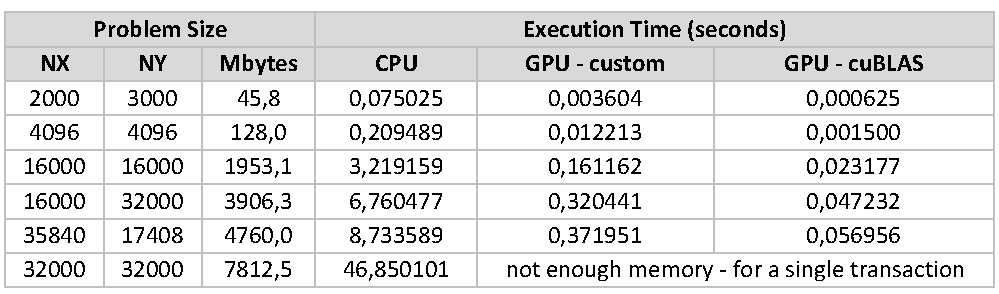
\includegraphics[scale=0.9]{./figures/2_tnv/new1}
\end{center}

\newpage
\noindent Στον πίνακα που ακολουθεί αναλύονται οι χρόνοι εκτέλεσης του υπολογισμού ανα kernel για τα διάφορα μεγέθη εισόδου:

\begin{center}
    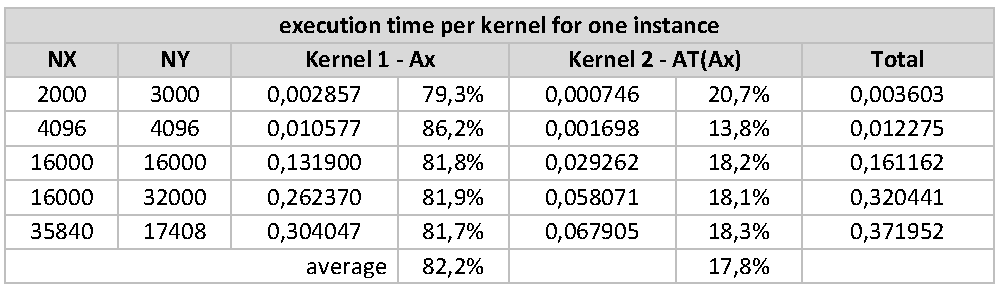
\includegraphics[scale=0.9]{./figures/2_tnv/new2}
\end{center}

\subsection*{Συμπεράσματα}
\addcontentsline{toc}{subsection}{Συμπεράσματα}

\begin{center}
    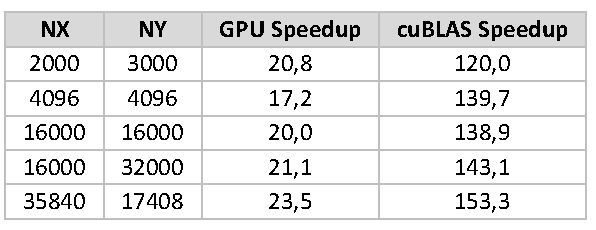
\includegraphics[scale=0.9]{./figures/2_tnv/speed_new}
\end{center}

\noindent Υπολογίζοντας τα μετρούμενα speedup τόσο της υλοποίησής μας όσο και της cuBLAS μπορούμε να οδηγηθούμε σε κάποια συμπεράσματα. Αρχικά ενώ έχουμε καταφέρει να πάρουμε αρκετά καλή βελτίωση της απόδοσης μέσω της δικής μας υλοποίησης γίνεται φανερό ότι χρήση της cuBLAS σε μία πιθανή εφαρμογή θα ήταν επιβεβλημένη, καθώς επιτυγχάνει εξαιρετική επιτάχυνση, ``εκτός ανταγωνισμού''.

\noindent Μπορούν να γίνουν οι εξής παρατηρήσεις:

\begin{enumerate}
    \item Όταν οι διαστάσεις του μεγέθους του μητρώου Α αποτελούν δυνάμεις του 2 ή πολλαπλάσια τους τότε έχουμε καλύτερα αποτελέσματα, από την άποψη μας ότι ο αλγόριθμος μας είναι πιο αποδοτικός. Ένας λόγος για τον οποίο μπορεί να συμβαίνει αυτό είναι ότι δημιουργούνται ομοιόμορφα grid και blocks στα οποία όλα τα thread αναλαμβάνουν αξιοποιούνται για τον υπολογισμό με αποτέλεσμα το μεγαλύτερο occupancy.
    
    \item Παρατηρούμε ότι ο δεύτερος kernel είναι σημαντικά ταχύτερος καθώς καταλαμβάνει μόνο το 10\% του συνολικού χρόνου κατά μέσο όρο, αν και φαινομενικά εκτελεί τον ίδιο υπολογισμό. Αυτό συμβαίνει καθώς πέρα από την χρήση της shared memory για την αποθήκευση του διανύσματος x εκμεταλλεύεται και την τεχνική του coalescing όταν προσπελαύνει τα στοιχεία του Α\textsuperscript{T} από την global memory.
\end{enumerate}


\subsection*{Περαιτέρω Βελτίωση}
\addcontentsline{toc}{subsection}{Περαιτέρω Βελτίωση}

\noindent Είναι φανερό ότι υπάρχουν μεγάλα περιθώρια βελτίωσης της απόδοσης της εφαρμογής μας τα οποία όμως ίσως ξεφεύγουν από τα πλαίσια της παρούσας εργασίας. Θα μπορούσαμε να τα συνοψίσουμε στα εξής σημεία:

\begin{itemize}
    \item Θα πρέπει να επικεντρωθούμε στην βελτίωση του πρώτου υπολογιστικού πυρήνα ο οποίος προσπελαύνει την global memory με μη-coalesced τρόπο με αποτέλεσμα την σημαντική επιβάρυνση του απαιτούμενου χρόνου. Μια ιδέα είναι να μεταφέρουμε τμήματα του μητρώου Α στην shared memory κατα την διάρκεια του υπολογισμού υλοποιώντας ουσιαστικά έναν \textbf{tiled shared memory} αλγόριθμο πολλαπλασιασμού μητρώου διανύσματος. Μία τέτοια προσέγγιση προτείνεται στην εργασία \cite{Erik:tiled}, την οποία αν και καταφέραμε και εντάξαμε στην υλοποίηση μας με πολύ καλά αποτελέσματα για τετραγωνικά μητρώα με διαστάσεις δυνάμεις του 2, δεν δούλευε για όλα τα μεγέθη εισόδου. Μια λύση θα ήταν να τροποποιήσουμε τον κώδικά μας ώστε να μετατρέπει το μητρώο εισόδου σε τετραγωνικό με μέγεθος κάθε διάστασης την κοντινότερη δύναμη του 2 για την μεγαλύτερη από τις 2 αρχικές.
    
    \item Το δεύτερο σημείο επικεντρώνεται στην παρατήρηση οτι η cuBLAS επιτυγχάνει εξαιρετικά αποτελέσματα. Καθώς πρόκειται για μια closed source βιβλιοθήκη της nVidia δεν έχουμε πρόσβαση στον κώδικα της ώστε να προσπαθήσουμε τον κατανοήσουμε τον τρόπο λειτουργίας της. Για τον λόγο αυτό αναζητήσαμε να βρούμε open source υλοποιήσεις της BLAS για GPU και να δούμε με ποιον τρόπο αντιμετωπίζουν την gemv. Πράγματι εντοπίσαμε την \href{https://github.com/ecrc/kblas-gpu/}{kblas-gpu} η οποία υλοποιεί τις \href{https://github.com/ecrc/kblas-gpu/tree/master/src/blas_l2}{level 2} συναρτήσεις της blas. Αν είχαμε περισσότερο χρόνο θα μπορούσαμε να μελετήσουμε και αυτήν την προσέγγιση για να δούμε αν θα πετυχαίναμε περαιτέρω βελτίωση.
    
    % \item Μία ακόμα ιδέα βελτιστοποίησης που προέκυψε τελευταία στιγμή είναι αντί να αντιμετωπίσουμε τον  πρώτο υπολογισμό ως έναν πολλαπλασιασμό
\end{itemize}

% Μία ιδέα βελτιστ

% \begin{center}
%     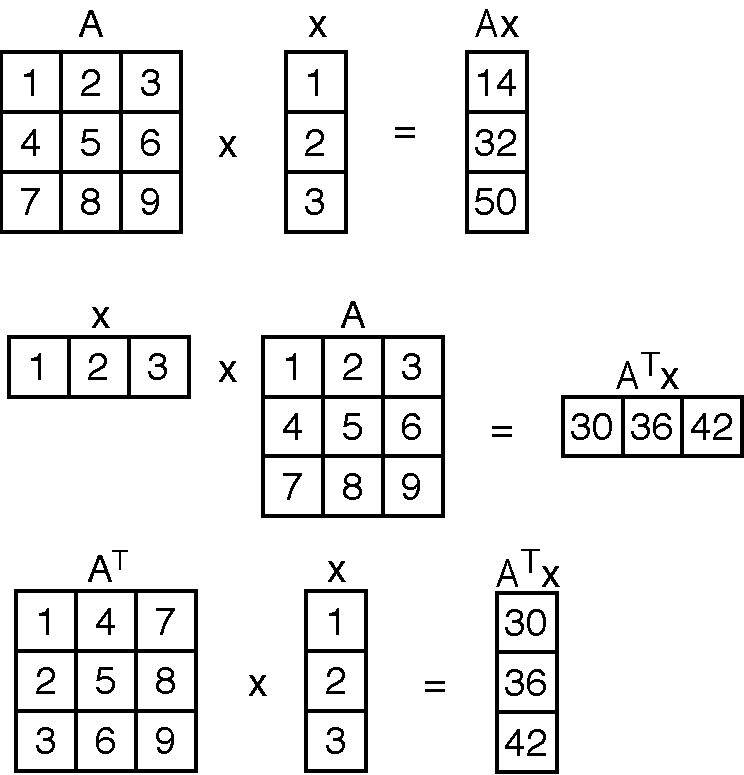
\includegraphics[scale=0.8]{./figures/2_tnv/mult}
% \end{center}


\newpage

\section{Covariance}
\noindent Η ανάλυση των περισσότερων μεθόδων και τεχνικών βελτιστοποίησης που χρησιμοποιήσαμε στα πλαίσια της εργασίας έχει ήδη αναφερθεί στα προηγούμενα ερωτήματα. Στη συνέχεια γίνεται μία σύντομη επισκόπηση του τρόπου με τον οποίο έγινε η παραλληλοποίηση στη GPU του κώδικα του τρίτου ερωτήματος. 

\noindent Στο συγκεκριμένο ερώτημα υπολογίζεται το μητρώο συνδιακύμανσης ενός αρχικού μητρώου μεγέθους \mbox{M X N}. Ο υπολογισμός αυτός γίνεται σε τρία βήματα:

\begin{enumerate}
    \item \textbf{Mean Calculation:} Για κάθε στήλη του μητρώου Α υπολογίζεται ο μέσος όρος των στοιχείων της στήλης.
    
    \item \textbf{Matrix Centering:} Από κάθε στοιχείο κάθε στήλης του μητρώου αφαιρεί τον μέσο όρο της αντίστοιχης στήλης που υπολογίστηκε στο προηγούμενο βήμα.
    
    \item \textbf{Covariance Matrix Calculation:} Πολλαπλασιάζεται το μητρώο που υπολογίστηκε στο προηγούμενο βήμα με το ανάστροφό του. Επειδή το αποτέλεσμα που προκύπτει είναι συμμετρικό μητρώο, αρκεί ο υπολογισμός είτε του άνω είτε του κάτω τριγωνικού μέρους του.
    
    
\end{enumerate}

\subsection*{CUDA-naïve implementation}
\addcontentsline{toc}{subsection}{CUDA-naïve implementation}

\noindent Αρχικά προχωρήσαμε στην απλούστερη δυνατή μορφή παραλληλοποίησης του κώδικα που μας δίνεται, δημιουργώντας έναν υπολογιστικό πυρήνα για κάθε ένα από τα βήματα του υπολογισμού όπως αυτά αναφέρθηκαν παραπάνω. Επίσης δημιουργήθηκε και μία συνάρτηση wrapper η οποία αναλαμβάνει να υπολογίσει τις κατάλληλες παραμέτρους και να καλέσει κάθε kernel.

\begin{enumerate}
    \item \textbf{\texttt{\textunderscore\textunderscore global\textunderscore\textunderscore\  void mean\textunderscore kernel(double *mean\textunderscore d, double *data\textunderscore d)}}
    
    \item \textbf{\texttt{\textunderscore\textunderscore global\textunderscore\textunderscore\  void reduce\textunderscore kernel(double *mean\textunderscore d, double *data\textunderscore d)}}
    
    \item \textbf{\texttt{\textunderscore\textunderscore global\textunderscore\textunderscore\  void covar\textunderscore kernel(double *symmat\textunderscore d, double *data\textunderscore d)}}
    
    \item \textbf{\texttt{\textunderscore\textunderscore host\textunderscore\textunderscore\  void calculate\textunderscore on\textunderscore GPU(...) // wrapper function}}
\end{enumerate}

Επόμενο βήμα είναι ο έλεγχος της ορθότητας των υπολογισμών ώστε να διαπιστώσουμε ότι το πρόγραμμα μας παράγει τα επιθυμητά αποτελέσματα. Για τον λόγο αυτό πέρα από την εγγραφή των αποτελεσμάτων στα αρχεία cpu.out και gpu.out έχει δημιουργηθεί η συνάρτηση \textittt{\textit{compareResults()}} η οποία συγκρίνει μεταξύ τους τα στοιχεία που παράχθηκαν στην CPU και την GPU και μετρά πόσα από αυτά διαφέρουν πάνω από ένα προκαθορισμένο ποσοστό σφάλματος. Η ιδέα αυτή προέρχεται από τον τρόπο με τον οποίο γίνεται η σύγκριση των αποτελεσμάτων στην υλοποίηση των PolyBench benchmarks για GPU όπως αυτά φαίνονται \href{http://web.cse.ohio-state.edu/~pouchet.2/software/polybench/GPU/index.html}{εδώ} και στην εργασία \cite{polybench}.


\subsection*{Βελτιστοποίηση}
\addcontentsline{toc}{subsection}{Βελτιστοποίηση}

\noindent Αφού επιβεβαιώσαμε την ορθότητα των υπολογισμών έγινε η βελτιστοποίηση του παράλληλου κώδικα. Επιτύχαμε πολύ μεγάλη εξοικονόμηση χρόνου με την χρήση καταχωρητών για την αποθήκευση των ενδιάμεσων αποτελεσμάτων. Με αυτόν τον τρόπο αντί να προσπελαύνεται πολλαπλές φορές η global memory απο κάθε thread, χρησιμοποιείται μία τοπική μεταβλητή για την αποθήκευση του αποτελέσματος και στην συνέχεια αυτό εγγράφεται στην global memory όταν έχει ολοκληρωθεί ο υπολογισμός του.

\pagebreak

\subsection*{Αποτελέσματα}
\addcontentsline{toc}{subsection}{Αποτελέσματα}

\noindent Παρακάτω συγκεντρώνονται τα αποτελέσματα επαναλαμβανόμενων εκτελέσεων του προγράμματος για διαφορετικά μεγέθη εισόδου.

\begin{center}
    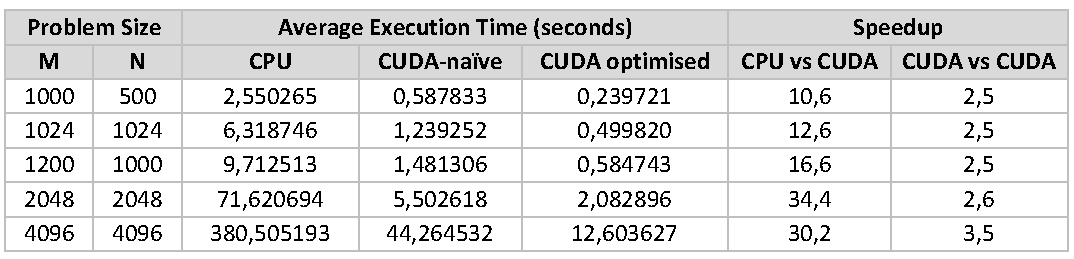
\includegraphics[scale=0.85]{./figures/3_covar/covar}
\end{center}

\noindent Το πρώτο speedup που υπολογίζεται αφορά την επιτάχυνση που δίνει ο βελτιωμένος κώδικας σε σχέση με την σειριακή εκτέλεση στη CPU. Το δεύτερο speedup αναφέρεται στην επιτάχυνση που έδωσαν οι βελτιστοποιημένοι cuda kernels σε σχέση με την naive εκδοχή τους. 

\subsection*{Συμπεράσματα}
\addcontentsline{toc}{subsection}{Συμπεράσματα}

Το πρώτο που παρατηρούμε είναι ότι η χρήση καταχωρητών αντί για προσπέλαση της global memory είναι απο μόνη της ικανή να μας δώσει πολύ μεγάλη βελτίωση του χρόνου εκτέλεσης. Επίσης γίνεται φανερό ότι όσο μεγαλώνει το μέγεθος του προβλήματος, τόσο μεγαλύτερο speedup επιτυγχάνεται που όμως μετά από ένα σημείο παραμένει σχετικά σταθερό.

\begin{center}
    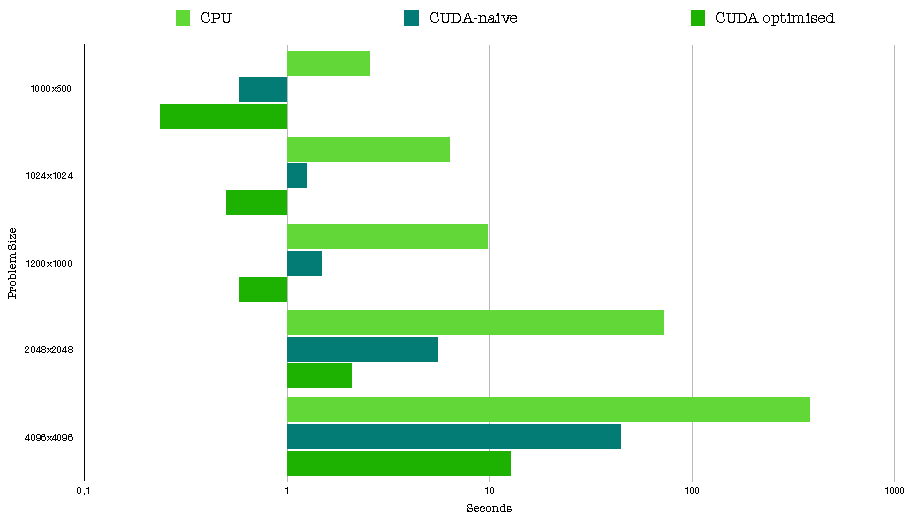
\includegraphics[scale=1]{./figures/3_covar/diag}
\end{center}

\newpage

\section{Google Cloud Platform}
\noindent Ως τελευταίο μέρος της εργασίας και περισσότερο για λόγους πειραματισμού, αποφασίσαμε να τρέξουμε τον κώδικα μας στην πλατφόρμα Google Cloud Platform αξιοποιώντας την πρόσβαση που μας παρέχει σε πιο σύγχρονο εξοπλισμό. Παρακάτω παρατίθενται τα τεχνικά χαρακτηριστικά του virtual machine που δημιουργήσαμε:

\begin{verbatim}
======== CPU ========
Architecture:          x86_64
CPU op-mode(s):        32-bit, 64-bit
Byte Order:            Little Endian
CPU(s):                4
On-line CPU(s) list:   0-3
Thread(s) per core:    2
Core(s) per socket:    2
Socket(s):             1
NUMA node(s):          1
Vendor ID:             GenuineIntel
CPU family:            6
Model:                 45
Model name:            Intel(R) Xeon(R) CPU @ 2.60GHz
Stepping:              7
CPU MHz:               2600.000
BogoMIPS:              5200.00
Hypervisor vendor:     KVM
Virtualization type:   full
L1d cache:             32K
L1i cache:             32K
L2 cache:              256K
L3 cache:              20480K

======== RAM ========
MemTotal:       16425608 kB

======== GPU ========
Device 0: "Tesla V100-SXM2-16GB"
  CUDA Driver Version / Runtime Version          10.0 / 10.0
  CUDA Capability Major/Minor version number:    7.0
  Total amount of global memory:                 16130 MBytes (16914055168 bytes)
  (80) Multiprocessors, ( 64) CUDA Cores/MP:     5120 CUDA Cores
  GPU Max Clock rate:                            1530 MHz (1.53 GHz)
  Memory Clock rate:                             877 Mhz
  Memory Bus Width:                              4096-bit
  L2 Cache Size:                                 6291456 bytes
  Maximum Texture Dimension Size (x,y,z)         1D=(131072), 2D=(131072, 65536), 
                                                 3D=(16384, 16384, 16384)
  Maximum Layered 1D Texture Size, (num) layers  1D=(32768), 2048 layers
  Maximum Layered 2D Texture Size, (num) layers  2D=(32768, 32768), 2048 layers
  Total amount of constant memory:               65536 bytes
  Total amount of shared memory per block:       49152 bytes
  Total number of registers available per block: 65536
  Warp size:                                     32
  Maximum number of threads per multiprocessor:  2048
  Maximum number of threads per block:           1024
  Max dimension size of a thread block (x,y,z): (1024, 1024, 64)
  Max dimension size of a grid size    (x,y,z): (2147483647, 65535, 65535)
  Maximum memory pitch:                          2147483647 bytes
  Texture alignment:                             512 bytes
  Concurrent copy and kernel execution:          Yes with 2 copy engine(s)
  Run time limit on kernels:                     No
  Integrated GPU sharing Host Memory:            No
  Support host page-locked memory mapping:       Yes
  Alignment requirement for Surfaces:            Yes
  Device has ECC support:                        Enabled
  Device supports Unified Addressing (UVA):      Yes
  Device supports Compute Preemption:            Yes
  Supports Cooperative Kernel Launch:            Yes
  Supports MultiDevice Co-op Kernel Launch:      Yes
  Device PCI Domain ID / Bus ID / location ID:   0 / 0 / 4
\end{verbatim}

\subsection*{Αποτελέσματα}

\noindent Παρακάτω παρατίθενται οι μετρήσεις που προέκυψαν από την εκτέλεση του κώδικα των δύο τελευταίων ερωτημάτων στο νέο περιβάλλον. Σε αυτό το σημείο πρέπει να αναφερθεί ότι δεν προχωρήσαμε σε βελτιστοποίηση του προγράμματος ώστε να ανταποκρίνεται καλύτερα στις πιθανές απαιτήσεις που θέτει η εκτέλεσή του σε μία αρκετά μεταγενέστερη κάρτα γραφικών, παραμόνο τρέξαμε τον ίδιο κώδικα για να δούμε πως θα συμπεριφερθεί στο νέο υλικό.

\begin{center}
    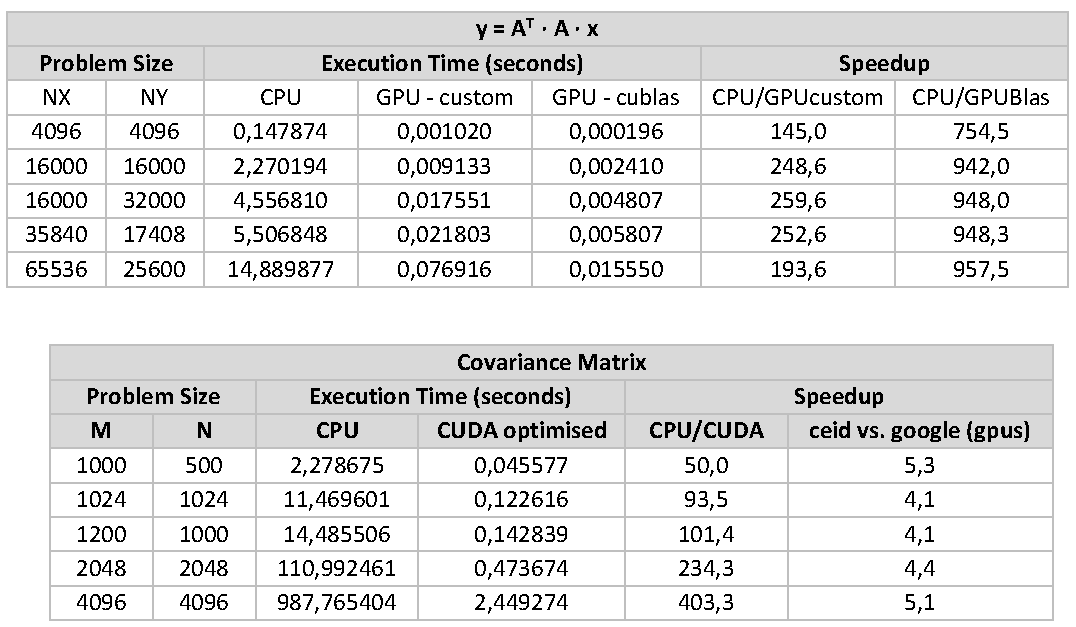
\includegraphics[scale=0.9]{./figures/3_covar/google}
\end{center}

\noindent Με μία πρώτη ματιά παρατηρούμε ότι και μόνο η μετάβαση σε μία πιο ισχυρή κάρτα γραφικών είναι ικανή να μας δώσει πολλαπλάσιο speedup από αυτό που πετυχαίναμε. Επίσης είναι φανερό ότι η κυριότερη διαφορά έγκειται στην επεξεργαστική ισχύ της GPU και όχι της CPU αφού σε πολλές περιπτώσεις ο αρχικός επεξεργαστής κατέληγε σε μικρότερους χρόνους εκτέλεσης. Τέλος, πολλά από τα αρχικά συμπεράσματα ισχύουν και σε αυτήν την περίπτωση καθώς και εδώ βλέπουμε την υπεροχή της cuBLAS σε σχέση με την δική μας υλοποίηση ενώ παρατηρούμε ότι σε γενικές γραμμές, όσο μεγαλύτερο είναι το μέγεθος του προβλήματος τόσο καλύτερο speedup παίρνουμε. 

\newpage

\bibliography{cuda} 
\addcontentsline{toc}{section}{Αναφορές}
\bibliographystyle{IEEEtran}

\end{document}




%kernel/system/do_fork.c

